% ---------------------------------------------------------------------------------------------------------------
% TEMPLATE PARA TRABALHO DE CONCLUSÃO DE CURSO
% Universidade Tecnológica Federal do Paraná - UTFPR
% Customização da classe abnTeX2 (http://www.abntex.net.br/) para as normas da UTFPR
%
% Autores: Diego Marczal
% 	       Michael Vornes <https://github.com/mvornes>
% Adaptação (DACOM-CP): Silvio Ricardo Rodrigues Sanches
%
%----------------------------------------------------------------------------------------------------------------
% Codificação: UTF-8
% LaTeX:  abnTeX2          
% ---------------------------------------------------------------------------------------------------------------


% CARREGA CLASSE PERSONALIZADA DA UTFPR--------------------------------------------------------------------------
\documentclass[%twoside,                   % Impressão em frente e verso
    	        oneside,                   % Impressão apenas frente
]{configuracoes/utfpr-abntex2}


% INCLUI ARQUIVOS DE CONFIGURAÇÕES-------------------------------------------------------------------------------
% REFERÊNCIAS------------------------------------------------------------------
\usepackage[%
    alf,
    abnt-emphasize=bf,
    bibjustif,
    recuo=0cm,
    abnt-url-package=url,       % Utiliza o pacote url
    abnt-refinfo=yes,           % Utiliza o estilo bibliográfico abnt-refinfo
    abnt-etal-cite=3,
    abnt-etal-list=3,
    abnt-thesis-year=final
]{abntex2cite}                  % Configura as citações bibliográficas conforme a norma ABNT

% PACOTES----------------------------------------------------------------------
\usepackage[utf8]{inputenc}                                 % Codificação do documento
\usepackage[T1]{fontenc}                                    % Seleção de código de fonte
\usepackage{booktabs}                                       % Réguas horizontais em tabelas
\usepackage{color, colortbl}                                % Controle das cores
\usepackage{float}                                          % Necessário para tabelas/figuras em ambiente multi-colunas
\usepackage{graphicx}                                       % Inclusão de gráficos e figuras
\usepackage{icomma}                                         % Uso de vírgulas em expressões matemáticas
\usepackage{indentfirst}                                    % Indenta o primeiro parágrafo de cada seção
\usepackage{microtype}                                      % Melhora a justificação do documento
\usepackage{multirow, array}                                % Permite tabelas com múltiplas linhas e colunas
\usepackage{subeqnarray}                                    % Permite subnumeração de equações
\usepackage{lastpage}                                       % Para encontrar última página do documento
\usepackage{verbatim}                                       % Permite apresentar texto tal como escrito no documento, ainda que sejam comandos Latex
\usepackage{amsfonts, amssymb, amsmath}                     % Fontes e símbolos matemáticos
\usepackage[algoruled, portuguese]{algorithm2e}             % Permite escrever algoritmos em português
%\usepackage[scaled]{helvet}                                % Usa a fonte Helvetica
\usepackage{times}                                          % Usa a fonte Times
%\usepackage{palatino}                                      % Usa a fonte Palatino
%\usepackage{lmodern}                                       % Usa a fonte Latin Modern
\usepackage[bottom]{footmisc}                               % Mantém as notas de rodapé sempre na mesma posição
\usepackage{ae, aecompl}                                    % Fontes de alta qualidade
\usepackage{latexsym}                                       % Símbolos matemáticos
\usepackage{lscape}                                         % Permite páginas em modo "paisagem"
%\usepackage{picinpar}                                      % Dispor imagens em parágrafos
%\usepackage{scalefnt}                                      % Permite redimensionar tamanho da fonte
%\usepackage{subfig}                                        % Posicionamento de figuras
%\usepackage{upgreek}                                       % Fonte letras gregas
\usepackage{adjustbox}                                      % Ajustar tamanho de tabelas
% Redefine a fonte para uma fonte similar a Arial (fonte Helvetica)
\renewcommand*\familydefault{\sfdefault}

% CONFIGURAÇÕES DE APARÊNCIA DO PDF FINAL--------------------------------------
\makeatletter
\hypersetup{%
    portuguese,
    colorlinks=true,   % true: "links" coloridos; false: "links" em caixas de texto
    linkcolor=blue,    % Define cor dos "links" internos
    citecolor=blue,    % Define cor dos "links" para as referências bibliográficas
    filecolor=blue,    % Define cor dos "links" para arquivos
    urlcolor=blue,     % Define a cor dos "hiperlinks"
    breaklinks=true,
    pdftitle={\@title},
    pdfauthor={\@author},
    pdfkeywords={abnt, latex, abntex, abntex2}
}
\makeatother

% ALTERA O ASPECTO DA COR AZUL--------------------------------------------------
\definecolor{blue}{RGB}{41,5,195}

% REDEFINIÇÃO DE LABELS---------------------------------------------------------
\renewcommand{\algorithmautorefname}{Algoritmo}
\def\equationautorefname~#1\null{Equa\c c\~ao~(#1)\null}

% CRIA ÍNDICE REMISSIVO---------------------------------------------------------
\makeindex

% HIFENIZAÇÃO DE PALAVRAS QUE NÃO ESTÃO NO DICIONÁRIO---------------------------
\hyphenation{%
    qua-dros-cha-ve
    Kat-sa-gge-los
}

\graphicspath{ {./dados/figuras/} }


% INCLUI ARQUIVOS DO TRABALHO DE CONCLUSÃO DE CURSO (PRÉ-TEXTUAIS, TEXTUAIS, PÓS-TEXTUAIS)-----------------------

% INSERE CAPA E FOLHA DE ROSTO
% CAPA---------------------------------------------------------------------------------------------------

% ORIENTAÇÕES GERAIS-------------------------------------------------------------------------------------
% Caso algum dos campos não se aplique ao seu trabalho, como por exemplo,
% se não houve coorientador, apenas deixe vazio.
% Exemplos: 
% \coorientador{}
% \departamento{}

% DADOS DO TRABALHO--------------------------------------------------------------------------------------
\titulo{Implementação de uma ferramenta para anotação de "Copy Number Variations" utilizando múltiplos algoritmos de "Change Point Detection"}
\titleabstract{Implementation a tool for annotation of Copy Number Variations using multiple algorithms of Change Point Detection}
\autor{Kássia Catarine Aires da Silva Lopes}
\autorcitacao{LOPES, Kássia} % Sobrenome em maiúsculo
\local{Cornélio Procópio}
\data{2019}

% NATUREZA DO TRABALHO-----------------------------------------------------------------------------------
% Opções: 
% - Trabalho de Conclusão de Curso (se for Graduação)
% - Dissertação (se for Mestrado)
% - Tese (se for Doutorado)
% - Projeto de Qualificação (se for Mestrado ou Doutorado)
\projeto{Trabalho de Conclusão de Curso}

% TÍTULO ACADÊMICO---------------------------------------------------------------------------------------
% Opções:
% - Bacharel ou Tecnólogo (Se a natureza for Trabalho de Conclusão de Curso)
% - Mestre (Se a natureza for Dissertação)
% - Doutor (Se a natureza for Tese)
% - Mestre ou Doutor (Se a natureza for Projeto de Qualificação)
\tituloAcademico{Bacharel}

% ÁREA DE CONCENTRAÇÃO E LINHA DE PESQUISA---------------------------------------------------------------
% Se a natureza for Trabalho de Conclusão de Curso, deixe ambos os campos vazios
% Se for programa de Pós-graduação, indique a área de concentração e a linha de pesquisa
\areaconcentracao{}
\linhapesquisa{}

% DADOS DA INSTITUIÇÃO-----------------------------------------------------------------------------------
% Se a natureza for Trabalho de Conclusão de Curso, coloque o nome do curso de graduação em "programa"
% Formato para o logo da Instituição: \logoinstituicao{<escala>}{<caminho/nome do arquivo>}
\instituicao{Universidade Tecnológica Federal do Paraná}
\departamento{Departamento Acadêmico de Computação}
\programa{Curso de Bacharelado Em Engenharia De Software}
\logoinstituicao{0.2}{dados/figuras/logo-instituicao} 

% DADOS DOS ORIENTADORES---------------------------------------------------------------------------------
\orientador{André Yoshiaki Kashiwabara}
%\orientador[Orientadora:]{Nome da orientadora}
\instOrientador{UTFPR - CP}

% \coorientador{Nome do coorientador}
%\coorientador[Coorientadora:]{Nome da coorientadora}
% \instCoorientador{Instituição do coorientador}

% FOLHA DE ROSTO--------------------------------------------------------------------------------------------------------

% TRABALHO DE CONCLUSÃO DE CURSO
 \preambulo{{\imprimirprojeto} apresentado ao {\imprimirprograma} da {\imprimirinstituicao}, como requisito parcial para a obtenção do título de {\imprimirtituloAcademico}.}

% DISSERTAÇÃO DE MESTRADO
% \preambulo{{\imprimirprojeto} apresentada ao Programa de \mbox{Pós-graduação} da {\imprimirinstituicao}, como requisito parcial para obtenção do título de {\imprimirtituloAcademico}.}

% TESE DE DOUTORADO
% \preambulo{{\imprimirprojeto} apresentada ao Programa de \mbox{Pós-graduação} da {\imprimirinstituicao}, como requisito parcial para a obtenção do título de {\imprimirtituloAcademico}.}

% PROJETO DE QUALIFICAÇÃO DE MESTRADO OU DOUTORADO
%\preambulo{{\imprimirprojeto} apresentado ao Programa de \mbox{Pós-graduação} da {\imprimirinstituicao}, como requisito parcial para a obtenção do título de {\imprimirtituloAcademico}.}

% OBSERVAÇÕES-----------------------------------------------------------------------------------------------------------
% Altere este arquivo APENAS comentando as linhas que não se aplicam ao tipo de trabalho acadêmico desejado.


\begin{document}

\pretextual
\imprimircapa                                               	           % Comando para imprimir Capa
\imprimirfolhaderosto{}                                     		   % Comando para imprimir Folha de rosto
% INSERE ELEMENTOS PRÉ-TEXTUAIS
% DEDICATÓRIA------------------------------------------------------------------

\renewcommand{\dedicatorianame}{DEDICATÓRIA}

\begin{dedicatoria}

Altere este texto inserindo a dedicatória do seu trabalho. 

\end{dedicatoria}
          			   % Dedicatória
% AGRADECIMENTOS---------------------------------------------------------------

\begin{agradecimentos}[AGRADECIMENTOS]

Edite e coloque aqui os agradecimentos às pessoas e/ou instituições que contribuíram para a realização do trabalho.

É obrigatório o agradecimento às instituições de fomento à pesquisa que financiaram total ou parcialmente o trabalho, inclusive no que diz respeito à concessão de bolsas.

\end{agradecimentos}
        			   % Agradecimentos
% EPÍGRAFE---------------------------------------------------------------------

\renewcommand{\epigraphname}{EPÍGRAFE}

\begin{epigrafe}

\textit{Eu denomino meu campo de Gestão do Conhecimento, mas você não pode gerenciar conhecimento. Ninguém pode. O que pode fazer - o que a empresa pode fazer - é gerenciar o ambiente que otimize o conhecimento. (PRUSAK, Laurence, 1997).}

\end{epigrafe}

% OBSERVAÇÕES------------------------------------------------------------------
% Altere o texto para inserir a epígrafe do seu trabalho
              			   % Epígrafe
% RESUMO--------------------------------------------------------------------------------

\begin{resumo}[RESUMO]
\begin{SingleSpacing}

% Não altere esta seção do texto--------------------------------------------------------
\imprimirautorcitacao. \imprimirtitulo. \imprimirdata. \pageref {LastPage} f. \imprimirprojeto\ – \imprimirprograma, \imprimirinstituicao. \imprimirlocal, \imprimirdata.\\
%---------------------------------------------------------------------------------------

% Definir -- tema
A variação no número de cópia (Copy Number Variation/CNV) é uma alteração estrutural caracterizada pela inserção e/ou deleção de uma determinada região do genoma humano.
% Importância -- tema
A análise de CNVs é um fator relevante cientificamente, em razão de as variações ocorridas no genoma serem um dos fatores que contribuem para as características genéticas e o surgimento de doenças mendelianas.
% Descrever como elas podem ser vistas -- tema
As tecnologias de sequenciamento do DNA, são capazes de extrair as informações necessárias para que a análise e identificação de CNVs possa ser realizada. \\
% Descrever como elas podem ser detectadas -- tema
% Descrever do que se trata o trabalho -- Objetivo
% Como ele irá ser feito -- método
% O que foi feito -- resultado
% O que se conclui a partir disso -- conclusão


% Antigo
% A análise de variações no número de cópias (CNV) é uma das principais fontes de estudo acerca de doenças e características genéticas. As tecnologias de sequenciamento desenvolvidas permitiu a aplicação de métodos estatísticos, como a detecção de pontos de mudanças (CPD) em seus dados. A técnica de CPD pode determinar variações ocorridas em uma série temporal, identificando as suas localidades, ao aplicar cálculos de acordo com o algoritmo imposto. Propõe-se nesse projeto buscar fornecer uma nova ferramenta de detecção de CNVs com adaptações de vários métodos de CPD, para a leitura de linhas celulares, a partir de dados sequenciados do exoma. \\

\textbf{Palavras-chave}: Variação no número de cópia (Copy Number Variation/CNV). Change Point Detection (CPD). Análise de sequenciamento completo do exoma (WES).

\end{SingleSpacing}
\end{resumo}

% OBSERVAÇÕES---------------------------------------------------------------------------
% Altere o texto inserindo o Resumo do seu trabalho.
% Escolha de 3 a 5 palavras ou termos que descrevam bem o seu trabalho 
             			   % Resumo em Português
% ABSTRACT--------------------------------------------------------------------------------

\begin{resumo}[ABSTRACT]
\begin{SingleSpacing}

% Não altere esta seção do texto--------------------------------------------------------
\imprimirautorcitacao. \imprimirtitleabstract. \imprimirdata. \pageref {LastPage} f. \imprimirprojeto\ – \imprimirprograma, \imprimirinstituicao. \imprimirlocal, \imprimirdata.\\
%---------------------------------------------------------------------------------------

The analysis of copy number variation (CNV) is one of the main sources of study about diseases and genetic characteristics. The sequencing technologies developed allowed the application of statistical methods, such as the detection of change points (CPD) in their data. The CPD technique can determine variations occurring in a time series, identifying their localities, when applying calculations according to the imposed algorithm. In this project we propose to provide a new CNV detection tool with adaptations of various CPD methods for the reading of cell lines from sequenced exome data. \\

\textbf{Keywords}: Copy Number Variation (CNV). Change Point Detection (CPD). Analysis of whole exome sequencing (WES).

\end{SingleSpacing}
\end{resumo}

% OBSERVAÇÕES---------------------------------------------------------------------------
% Altere o texto inserindo o Abstract do seu trabalho.
% Escolha de 3 a 5 palavras ou termos que descrevam bem o seu trabalho 
             		           % Resumo em Inglês
% Lista de Figuras----------------------------------------------------------------

\pdfbookmark[0]{\listfigurename}{lof}
\listoffigures*
\cleardoublepage

% OBSERVAÇÕES---------------------------------------------------------------------
% Este arquivo não precisa de ser alterado, pois a lista é gerada automaticamente.
   % Lista de Figuras
% LISTA DE QUADROS----------------------------------------------------------------

\renewcommand{\listofquadrosname}{LISTA DE QUADROS}

\pdfbookmark[0]{\listofquadrosname}{loq}
\listofquadros*
\cleardoublepage

% OBSERVAÇÕES---------------------------------------------------------------------
% Este arquivo não necessita de ser editado. A lista é gerada automaticamente.
   % Lista de Quadros
% LISTA DE TABELAS-------------------------------------------------------------

\pdfbookmark[0]{\listtablename}{lot}
\listoftables*
\cleardoublepage

% OBSERVAÇÕES-------------------------------------------------------------------
% Este arquivo não precisa ser alterado, pois a lista é gerada automaticamente.
         		   % Lista de Tabelas
% LISTA DE ABREVIATURAS E SIGLAS----------------------------------------------------------

\begin{siglas}
    \item[DNA] Deoxyribonucleic Acid
    \item[RNA] Ribonucleic Acid
    \item[NGS] Next-Generation Sequencing
    \item[CNV] Copy Number Variation
    \item[CPD] Change Point Detection
    \item[TS] Time Series
    \item[AC] Acurácia
    \item[PC] Precisão
    \item[SB] Sensibilidade
    \item[Fscore] F-Score
\end{siglas}

% OBSERVAÇÕES-----------------------------------------------------------------------------
% Altere a lista acima para definir os acrônimos e siglas utilizados neste trabalho
          		   % Lista de Abreviaturas e Siglas
% LISTA DE SÍMBOLOS------------------------------------------------------------

\begin{simbolos}
    \item[$ \infty $] Infinito
    \item[$ \beta $] Letra grega Beta
    \item[$ \Gamma $] Letra grega Gama
    \item[$ \tau $] Letra grega Tau
    \item[$ \theta $] Letra grega Teta
    % \item[$ \in $] Pertence
\end{simbolos}

% OBSERVAÇÕES-------------------------------------------------------------------
% Altere a lista acima para definir os símbolos utilizados no trabalho
        		   % Lista de Símbolos
% LISTA DE ALGORITMOS----------------------------------------------------------

\newcommand{\algoritmoname}{Algoritmo}
\renewcommand{\listalgorithmcfname}{LISTA DE ALGORITMOS}

\floatname{algocf}{\algoritmoname}
\newlistof{listofalgoritmos}{loa}{\listalgoritmoname}
\newlistentry{algocf}{loa}{0}

\counterwithout{algocf}{chapter}
\renewcommand{\cftalgocfname}{\algoritmoname\space}
\renewcommand*{\cftalgocfaftersnum}{\hfill--\hfill}

\pdfbookmark[0]{\listalgorithmcfname}{loa}
\listofalgorithms
\cleardoublepage

% OBSERVAÇÕES------------------------------------------------------------------
% Este arquivo não precisa ser alterado, pois a lista é gerada automaticamente.
   % Lista de Algoritmos
% SUMÁRIO----------------------------------------------------------------------

\renewcommand{\contentsname}{SUMÁRIO}

\pdfbookmark[0]{\contentsname}{toc}
\tableofcontents*
\cleardoublepage

% OBSERVAÇÕES-------------------------------------------------------------------
% Este arquivo não precisa ser alterado, pois o sumário é gerado automaticamente.
                            % Sumário

\textual
% INSERE ELEMENTOS TEXTUAIS
% INTRODUÇÃO-------------------------------------------------------------------

\chapter{INTRODUÇÃO}
\label{chap:introducao}

% Importância de estudar o CNV
A variação no número de cópias (Copy Number Variation/CNVs) é um dos fatores que contribuem para a expansão e diversidade da família de genes, ela foi observada como alterações ocorridas em larga escada de inserções, deleções e duplicações na região genômica \cite{Perry2009,Zhao2013,Redon2006,Costain2016}. 
As CNVs podem ser identificada como uma variação neutra ou como modificadores de sucessibilidade a doenças \cite{Costain2016,Perry2009}.

% Estratégia de identificar CNV e ligação a doenças
A análise da região genômica pode ser realizada graças as tecnologias desenvolvidas para seu o sequenciamento, permitindo a observação de variantes de DNA \cite{Sathirapongsasuti2011}. Embora o sequenciamento completo do genoma seja uma abordagem utilizada para a investigação de CNVs, uma estratégia mais viável, econômica e eficiente no tempo para o estudo da base genética da doença é o sequenciamento completo do exoma, sendo que 85\% dos variantes ligados a doenças mendelianas são encontrados nele \cite{Chong2015,Sathirapongsasuti2011,Fromer2012}.

% Ligação aos modelos estatísticos
Devido a quantidade, complexidade e ruído dos dados obtidos a partir sequenciamento das regiões codificantes do genoma (exoma), muitos ferramentas de detecção de CNVs foram desenvolvidos para determinar os tipos, quantidades e a localização de variações \cite{Fromer2012,Tan2014}. Esses fatores foram alcançados devido a utilização de modelos estatísticos na descoberta de variações no mapa de dados gerados no sequenciamento do exoma, essa é uma das abordagens que obteve mais sucesso na integração das ferramentas com o sequenciamento devido a sua eficiência \cite{Tan2014}.

A utilização de modelos estatísticos aplicados para detecção de \textit{copy number variation} visa encontrar pontos de mudanças em uma representação gráfica dos dados, assim facilitando a determinação de uma variação de acordo com a localização do ponto de mudança \cite{Zhao2013}. Essa técnica se tornou popular, sendo desenvolvidos diversas ferramentas que detecta pontos de mudanças (Change Point Detection/CPD) focadas na análise de CNV \cite{Olshen2004,Baldi2001,Girimurugan2018,Picard2011,Plagnol2012,Muggeo2010}. 

Apesar das diversas técnicas e ferramentas existentes de CPD, nenhuma delas é capaz de identificar todas as CNVs presentes no exoma \cite{Zhao2013}, entretanto a utilização de algumas dessas técnicas em determinada situação alcança uma maior efetividade ao encontrar as variações. Essa diferença entre as técnicas pode ser vista ao comparar a execução de cinco algoritmos específicos de detecção de variações no números de cópias na \autoref{fig:ferramentas-cnv} \cite{Muggeo2010}.

\begin{figure}[!htb]
    \centering
    \caption{Segmentação da linha celular de câncer de mama MDA157, onde cada linha representa um cromossomo, indexado ao lado esquerdo}
    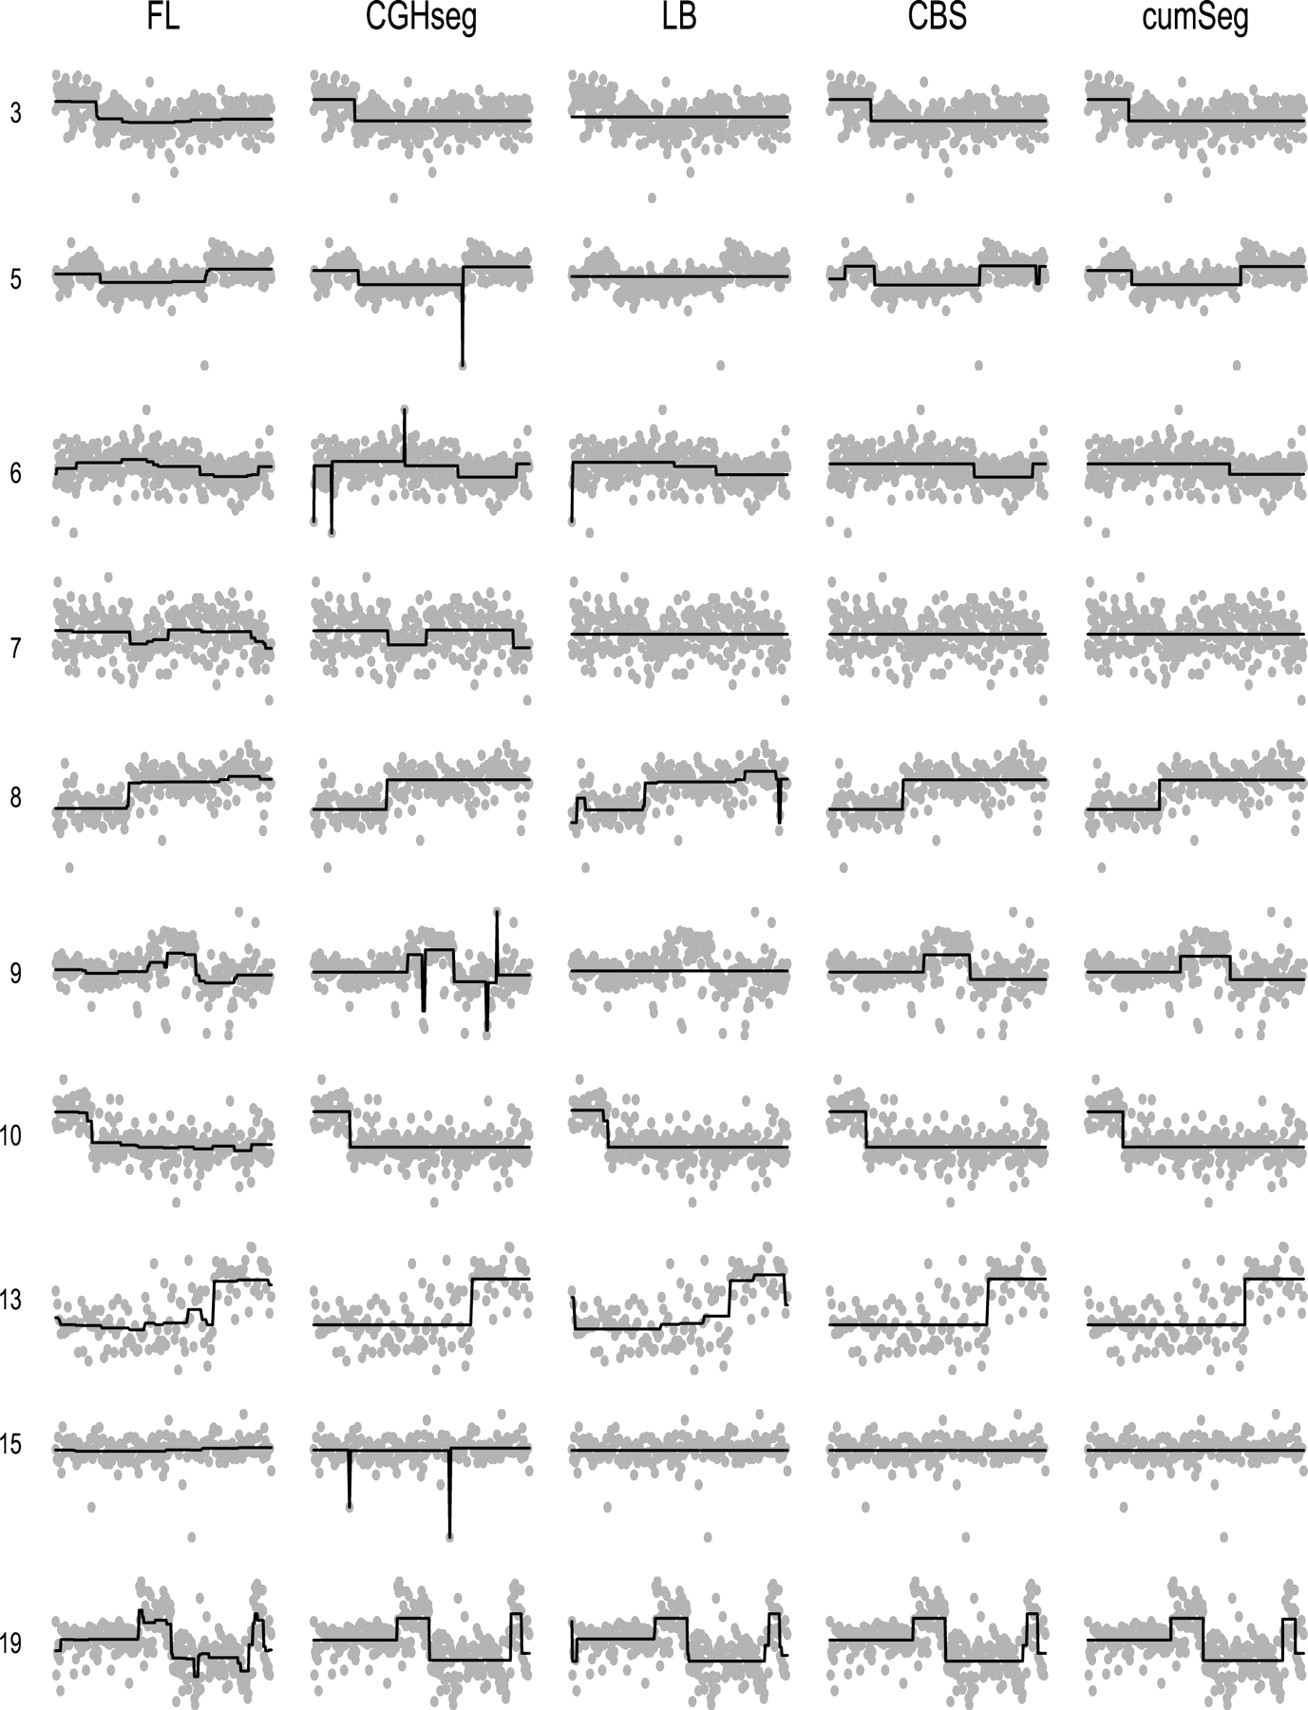
\includegraphics[width=0.8\textwidth]{./dados/figuras/ferramentas-cnv}
    \fonte{\cite{Muggeo2010}}
    \label{fig:ferramentas-cnv}
\end{figure}


% Contextualizar do estudo de CNV

% O genoma é uma grande fonte de informações acerca das nossas características e hereditariedade \cite{Correa2008}. O estudo das pequenas frações de regiões codificadoras de proteína do genoma (exoma) é bastante importante para a análise de doenças de origem genética, pois nele é contido cerca de 85\% de variantes conhecidos ligados a doenças \cite{Chong2015}.

% O exoma pode ser extraído por meio de um sequenciamento, onde seus variantes ficam visíveis para aplicação de algoritmos de análises e estudo de especialistas (referencia). O avanço tecnológico para detecção de padrões e anomalias nos dados gerados a parti do exoma tem-se evoluído ao longo do tempo, permitindo a observação das variações dos números de cópias (CNV) de cromossomos no DNA (referencia).

% A partir do sequenciamento do exoma é possível realizar uma distribuição dos dados mapeados em um gráfico, assim originando uma série temporal, ou seja, um conjunto de dados distribuídos ao longo de um determinado tempo (referencia). Desta forma, aumentando viabilidade de se analisar o CNV em determinadas posições.

% O Copy Number Variation (CNV) é observado quando ocorre alguma inserção ou deleção no cromossomo, fazendo com que ele deixe de ser diploide (referencia). Com a distribuição do dataset gerado pelo sequenciamento do exoma em um gráfico, os CNV ficam visíveis para serem estudados, mas a identificação do ponto onde ocorre algum tipo de CNV não é fácil de ser apontado e ou classificado, assim dificultando o apontamento de doenças genéticas.

% O reconhecimento da mudança ou ponto de mudança com uma maior precisão é um dos grandes desafios relacionado a análise estatística (referencia). O CP é fundamental para dar continuidade em pesquisas relacionadas a doenças ocorridas por algum CNV (referencia).

% O \textit{Change Point} é pouco perceptível a olho nu, dificultando o seu reconhecimento com uma maior precisão. Embora haja algoritmos que o detectam, como por exemplo \textit{Circular Binary Segmentation} ele não possui uma performance adequada para analise das segmentações mais recentes, pois elas contém uma quantidade imensa de marcadores assim aumentando o número de cálculos necessários para identificar a mudança em um determinado ponto por causa do uso de permutação em seu algoritmo.

% No meio estatístico, existe a utilização e implementação de diversos cálculos para solucionar tal questão, como  

% Diante das questões expostas, a exploração de novas algoritmos capaz de demonstrar uma melhor apresentação para detectar o CP vem sendo estudada, tanto no meio da estatística quanto no da bioinformática (referencia). Mas com a evolução e melhora das tecnologias, temos cada vez mais nitidez nas extração dos dados do exoma, assim necessitando de algoritmos e técnicas mais potentes para inspeção.

\section{JUSTIFICATIVA}



\section{OBJETIVOS}

Nesta seção será apresentado os objetivos que esse trabalho busca ao ser desenvolvido, sendo composto pelo objetivo geral e específico.

\subsection{Objetivo Geral}

Aplicar o conceito de detecção de pontos de mudanças, utilizando diferentes abordagens técnicas desenvolvidas para segmentação de dados de uma série temporal para anotação de variações no números de cópias nos dados do sequenciamento do exoma.

\subsection{Objetivos Específicos}
	
\begin{itemize}
    \item Explicar a importância de \textit{copy number variation}.
    \item Descrever o conceito de \textit{change point detection}, caracterizando com exemplos, os algoritmos desenvolvidos para esse objetivo.
    \item Analisar a aplicabilidade dos algoritmos de CPD para a CNV, citando exemplos dos mesmos.
\end{itemize}

\section{ORGANIZAÇÃO DO TEXTO}

Este trabalho se organiza da seguinte forma:

\autoref{chap:introducao} - Introdução: Situa o leitor na área de pesquisa em que o trabalho é focado, definindo o porque do seu desenvolvimento e os objetivos a serem alcançados com a conclusão do projeto.

\autoref{chap:fundamentacaoTeorica} - Revisão de Literatura: Apresenta uma pesquisa que contém conceitos e reflexões acerca dos principais conceitos referente ao trabalho proposto. Nele é apresentado temas relacionado ao trabalho proposto como a definição de exoma e a importância da utilização dele para descobertas de doenças (\autoref{sec:exoma}), o estudo acerca do surgimento e a evolução de tecnologias capazes de obter os componentes do genoma (\autoref{sec:sequenciamentoDoDna}), a definição de CNVs, ressaltando a importância do estudo e o uso dos métodos e ferramentas de detecção nessa variação genética (\autoref{sec:copyNumberVariation}), a formulação de uma das estratégias de detecção de CNV, a detecção de pontos de mudanças, sendo apresentado algoritmos específicos para utilização nesse tipo de situação (\autoref{sec:changePointDetection}) e a conceituação de matriz de confusão para aplicação em estudos com o objetivo de analise de performance \autoref{sec:matrizDeConfusao}.

\autoref{chap:planoDeTrabalho} - Plano de Trabalho: Expõe o cronograma adotado para o desenvolvimento do trabalho, disponibilizando o inicio e fim de um conjunto de atividades e sua descrição.

\autoref{chap:conclusao} - Conclusão: Apresenta as considerações finais acerca do trabalho desenvolvido.                		           % Introdução
% REVISÃO DE LITERATURA--------------------------------------------------------

\chapter{REVISÃO DE LITERATURA}
\label{chap:fundamentacaoTeorica}

A base teórica necessária para a realização da pesquisa e o entendimento do estudo é apresentada nesse capítulo, destacando os conceitos de Exoma, Sequenciamento do DNA, \textit{Copy Number Variation}, \textit{Change Point Detection}, algoritmos relacionados a CPD, como o \textit{Circular Binary Segmentation}, \textit{Graph Spectrum}, PELT, entre outros. Além desses tópicos o trabalho apresenta a descrição de Matriz de Confusão e Sistema R. Esses conceitos apresentados possui a finalidade de reunir evidências e contribuições sobre o uso do processo de algoritmos de detecção de pontos de mudança no contexto de anotação de \textit{copy number variation} utilizando os conceitos do Sistema R em seu desenvolvimento.

\section{EXOMA}
\label{sec:exoma}

O genoma é constituído de regiões codificantes e não codificantes, elas denominadas como \textit{éxons} e \textit{íntrons} respectivamente. As regiões codificantes constituem-se de sequências de proteínas, elas representam cerca de 1\% do genoma \cite{Ng2009}.Na \autoref{fig:figura-exoma} é representado essas regiões presentes na estrutura do DNA e RNA, podendo identificar os \textit{éxons} como as áreas destacadas com uma camada colorida e os \textit{íntrons} em cada espaço existente entre as sequências dos \textit{éxons}.

\begin{figure}[!htb]
    \centering
    \caption{Exemplificação das regiões codificantes de proteínas (\textit{éxons} ou exoma) na estrutura do DNA e RNA}
    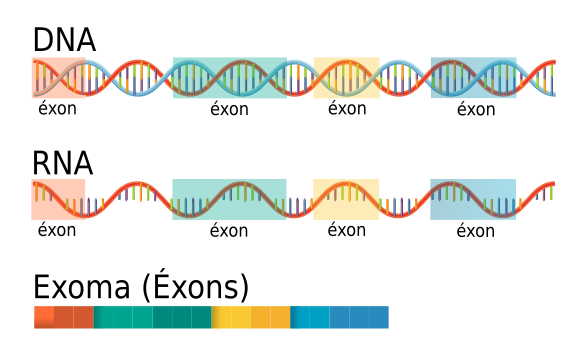
\includegraphics[width=0.8\textwidth]{./dados/figuras/exoma}
    \fonte{Autoria Própria}
    \label{fig:figura-exoma}
\end{figure}

A quantidade de 1\% do genoma pode chegar a conter aproximadamente 180 mil \textit{éxons}, esse conjunto de regiões codificantes de proteínas é conhecido como exoma, uma representação dele pode ser vista na \autoref{fig:figura-exoma} \cite{Bamshad2011}. O mesmo pode ser obtido pelo processo de sequenciamento completo do exoma, ele correspondente a separação dos \textit{éxons} contidos no genoma, o seu uso vem sendo registrado em demasiados diagnósticos moleculares de detecção de distúrbios genéticos, por ser possível identificar variantes relacionadas a doenças com as informações geradas \cite{Bamshad2011,Lee2014,HutchisonIII2007}. 

Apesar da aplicação do sequenciamento para obtenção do exoma através da extração dos \textit{éxons}, ainda existe dúvidas sobre quais regiões são exatamente codificantes de proteínas, assim não podendo ser especificado qual o exato conjunto equivalente ao exoma \cite{Bamshad2011}.

A utilização do teste de sequenciamento do exoma possibilitou um rendimento de 25-35\% em diagnósticos de doenças raras de origem genética \cite{Bamshad2011}. Entretanto, a utilização das informações produzidas não se contém a somente análise de distúrbios. Grandes esforços por parte de pesquisadores biomédicos, empresas de biotecnologia e medicamentos, agências financiadoras e grupos de pacientes, estão sendo direcionados na descoberta das funcionalidades, relações e reações que cada gene possui de acordo com alguma variação ao qual o mesmo foi disposto \cite{Antonarakis2006}. 

% Associar o exoma ao CNV 
O sequenciamento completo do exoma vem sendo utilizado em demasiados cenários oriundos de variações gênicas, como em descobertas de perda auditiva \cite{Likar2018}, encefalopatia epiléptica \cite{Allen2016}, mutação gerada a partir de uma determinada doença \cite{Lin2019}, hipotireoidismo congênito \cite{Fu2019}, entre outros. Essas pesquisas são realizadas em utilizando conjuntos de amostras de indivíduos com características semelhantes ou amostras com características extremamente opostas \cite{Bamshad2011}, para que sejam analisadas e comparadas, na tentativa de identificar onde alguma variação no número de cópias, que causa um determinado comportamento está situada encontra.

\section{SEQUENCIAMENTO DO DNA} 
\label{sec:sequenciamentoDoDna}

% Sobre o sequenciamento 
O estudo acerca do DNA e das informações contidas nele obteve um grande impulso por parte de vários cientistas do mundo inteiro no século XX, e com isso surgiu um movimento responsável pela investigação dos componentes do DNA, denominado como o Projeto Genoma Humano \cite{Lander2001}. Esse projeto levantou investimentos científico e capital, com um orçamento que variando entre US\$ 3 bilhões a US\$ 53 bilhões, para obter um maior entendimento das características do DNA a partir do sequenciamento completo do genoma \cite{Marian2011}. 

% Objetivo de sequenciamento 
Com o objetivo de ordenar os nucleotídeos do DNA, decodificando o código genético \cite{Edwards2011}, as primeiras pesquisas relacionadas ao sequenciamento surgiu próximo ao final do século XX, com variadas propostas acerca do assunto, uma delas foi a criação de tecnologias capazes de criar a sequencia completa do genoma humano, mapeando cada partícula existente \cite{Lander2001,HutchisonIII2007}. 

A tarefa de sequenciar o genoma humano completo consumou alguns anos para ser finalizada, sendo iniciada em 1990 e concluída oficialmente em 2003, apesar de conter mais de 5000 cientistas em centros de pesquisas do Estados Unidos, Europa e Japão, envolvidos no projeto \cite{HutchisonIII2007}, a sua conclusão tardia se deu por possuir uma certa complexidade ao montar e ordenar os pequenos pedaços sequenciados corretamente, além de possuir um enorme custo estimado em 3 bilhões de dólares para analise do conjunto de cadeias do DNA \cite{Rye2017,HutchisonIII2007}.

% Primeiro sequenciamento 
As tecnologias desenvolvidas para o sequenciamento tende a se desenvolver incrementalmente, utilizando algumas particularidades dos métodos existentes e melhorando-os conforme a necessidade da realidade atual \cite{HutchisonIII2007}. Entre os métodos pesquisados e desenvolvidos ao longo dos anos, o que mais se destacou no Projeto do Genoma Humano foi o método de Sanger, desenvolvido por volta de 1975 \cite{Sanger1975} e utilizado no sequenciamento completo do genoma humano \cite{HutchisonIII2007}, o seu sucesso se deu pela disponibilização de um alto nível de qualidade ao ler uma sequencia curta do DNA \cite{Edwards2011}. Ele possibilitou a análise dos segmentos do genoma vistos microscopicamente, como os cromossomos e as variações contidas em sua estrutura, usadas para visualizar as diferenças entre os genomas de amostras estudados \cite{Feuk2006,Sanger1975}. 

% Desvantagem e evolução do método/Explicar os modelos de sequenciamento https://www-nature.ez48.periodicos.capes.gov.br/articles/nrg2626#df3 
Apesar do sequenciamento de Sanger suprir as expectativas em sua época de sua criação e ainda ser utilizado em vários casos da atualidade, ele apresentava um custo elevado ao sequenciar genomas complexos, sendo estimado em 1 dólar por base de DNA sequenciada, o que dá em média 3 bilhões de dólares por genoma completo na época do projeto \cite{HutchisonIII2007}, esse fator ajudou a motivar o estudo de novos procedimentos capazes de obter aumento no desempenho e custos mais acessíveis em comparação com os existentes. 

A partir dessa realidade surgiu vários métodos baseados no \textit{next-genaration sequencing} (NGS), esses métodos são um conjunto de planos executados em conjunto para obter uma coleção maior de dados com um custo reduzido e melhor performance \cite{Metzker2010,Zhao2013}, como visto nos resultados produzidos pelos sequenciadores do Solexa \cite{Bennett2004}, HiSeq 2000, SOLID e outros \cite{Edwards2011,Linnarsson2010}. Esses equipamentos estão possibilitando uma maior cobertura e resolução, assim sendo possível identificar mais variações no número de cópias do genoma \cite{Zhao2013}. 

% Explicação técnica de como sequencia? 

% Introdução a análise computacional 
O início da análise computacional dos dados de sequenciamento foi abordado por Duncan McCallum e Michael Smith \cite{McCallum1977}, ao desenvolver um dos primeiros programas direcionados a compilação e estudo das informações sequenciadas \cite{HutchisonIII2007}. Entretanto, a criação de programas computacionais não se deteve com a evolução das técnicas de sequenciamento, assim sendo estudado e desenvolvidos novas formas de observações automatizadas para acompanhar a trajetória evolutiva das ferramentas de sequenciamento do DNA. 

% Explicar os dados gerados Dataset e como estão disponíveis 

\section{COPY NUMBER VARIATION} 
\label{sec:copyNumberVariation}

% Introdução ao assunto do CNV 
A \textit{copy number variation} (CNV) ou no português variação no número de cópias, são alterações que ocorrem na região genômica, elas se classificam como inserções, duplicações e deleções na estrutura do cromossomo, como representado na \autoref{fig:figura-copy-number-variation} \cite{Zhao2013,Redon2006}. Essas variações podem ser encontradas em todos os seres humanos, podendo não representar nenhuma alteração ou ser responsável por doenças de origem mendeliana, sua existência e descoberta são essenciais para o entendimento da composição genômica \cite{Redon2006,Feuk2006}.

% Definição de CNV com imagem
\begin{figure}[!htb]
    \centering
    \caption{Exemplo de variação no número de cópias (CNV) no cromossomo}
    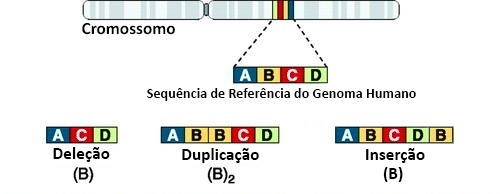
\includegraphics[width=1\textwidth]{./dados/figuras/copy-number-variation}
    \fonte{Adaptado de \cite{Dierssen2009}}
    \label{fig:figura-copy-number-variation}
\end{figure}

% Contexto 
Com o estudo do genoma humano \cite{Lander2001} houve a possibilidade de descobertas relevantes sobre doenças ao comparar a composição do DNA de várias pessoas, entretanto inicialmente essas descobertas se deu no nível macro, como em números de cromossomos. Portanto, a maior parte das doenças encontradas estavam relacionadas a análise do genoma completo, onde podiam ser vistos a partir de um microscópio \cite{Feuk2006}. 

As tecnologias de sequenciamento do DNA possibilitou a investigação das micropartículas que concebiam o genoma, a partir dela foi possível identificar a existência de pequenas inserções, deleções, inserções e duplicações não identificadas a partir de análises microscópica. De acordo com o estudo dessas variações no número de cópias da estrutura genômica foram vistos uma série de casos onde não representava nenhuma consequência e outros que possuíam uma grande chance de causar doenças de origem mendelianas \cite{Feuk2006,Xi2011}. 

% Sobre o estudo 
O estudo do CNV foi pouco aprofundado até recentemente em comparação com outras classes da variação genética \cite{Redon2006}, mas com o avanço do NGS e o auto rendimento produzido pelos sequenciamentos utilizados, houve um aumento no grau de avaliabilidade dos mesmos, sendo possível o reconhecimento das regiões afetadas, assim mudando essa realidade \cite{Mills2011,Feuk2006}.

As distribuições de variações do número de cópias se distinguem entre populações, elas são formadas por mutação, seleção e histórico demográfico, onde indivíduos que se encontram expostos a determinadas características, como por exemplo demográfica, apresentam variações semelhantes, assim sendo possível a identificação e classificação entre tipos de populações existentes \cite{Redon2006}. 

Em \cite{Snijders2001} é feita uma montagem de dados genômicos, a fim de mostrar as variações existentes e as suas medições precisas em um array CGH de uma amostra sequenciada pelo \textit{Coriell Institute for Medical Research}. Os dados dessa amostra, serão denominados como Coriell neste trabalho pela ligação com o instituto pesquisado, ela é utilizada em pesquisas por oferecer medições confiáveis das variações ocorridas. 

As alterações nos números de cópias apresentadas em Coriell, atende a várias origens, inclusive a variações recorrentes a câncer. Os microarrays montados graficamente a partir dos dados sequenciados é a relação de razão logarítmica média $_2$ (razão de $log_{2}$) pela posição ou pelo cromossomo, como apresentado na \autoref{fig:coriell-cnv}.

\begin{figure}[!htb]
    \centering
    \caption{Dados genômicos da amostra de DNA pertencente ao Coriell, referente a linhagem celular GM03576}
    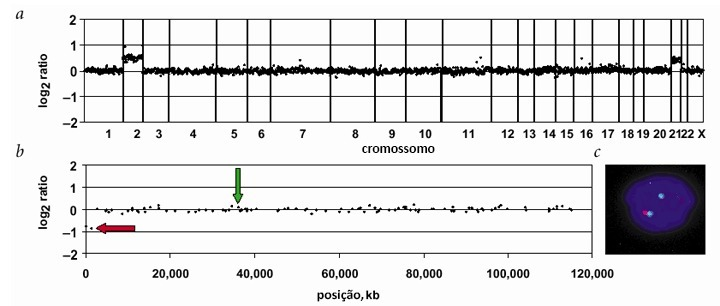
\includegraphics[width=1\textwidth]{./dados/figuras/coriell-cnv}
    \fonte{Adaptado de \cite{Snijders2001}}
    \label{fig:coriell-cnv}
\end{figure}

Uma linhagem celular GM03576, pertencente ao conjunto de dados do Coriell, demonstra a identificação de CNVs de acordo com a representação gráfica. A \autoref{fig:coriell-cnv}-a denota o ganho de números de cópias do cromossomo 2 e 21, onde é possível ver um aumento na média da razão de $log_{2}$. A \autoref{fig:coriell-cnv}-b destaca a deleção de números de cópias de acordo com o cromossomo 9 da linhagem celular apresentada, onde contém setas de identificação. 

O \cite{Snijders2001}, apresenta uma confirmação dos ganhos e perdas relatados acima, na \autoref{fig:coriell-cnv}-c, destacando os ganhos como pontos na cor verde e a perda como pontos na cor vermelha.

\subsection{Métodos de Detecção} 

A fim de estudar e descobrir as principais características acerca das regiões do genoma, sendo elas a codificante e a não codificante, a investigação da detecção das variações no número de cópias é essencial para o processo de descoberta de peculiaridades relacionadas a amostra. Para alcançar esse objetivo, \cite{Zhao2013} descreve existe cinco estratégias diferentes a serem aplicadas na detecção, sendo elas as detalhadas na \autoref{fig:estrategias-deteccao-cnv}.

\begin{figure}[!htb]
    \centering
    \caption{Estratégias de detecção de variações no número de cópias}
    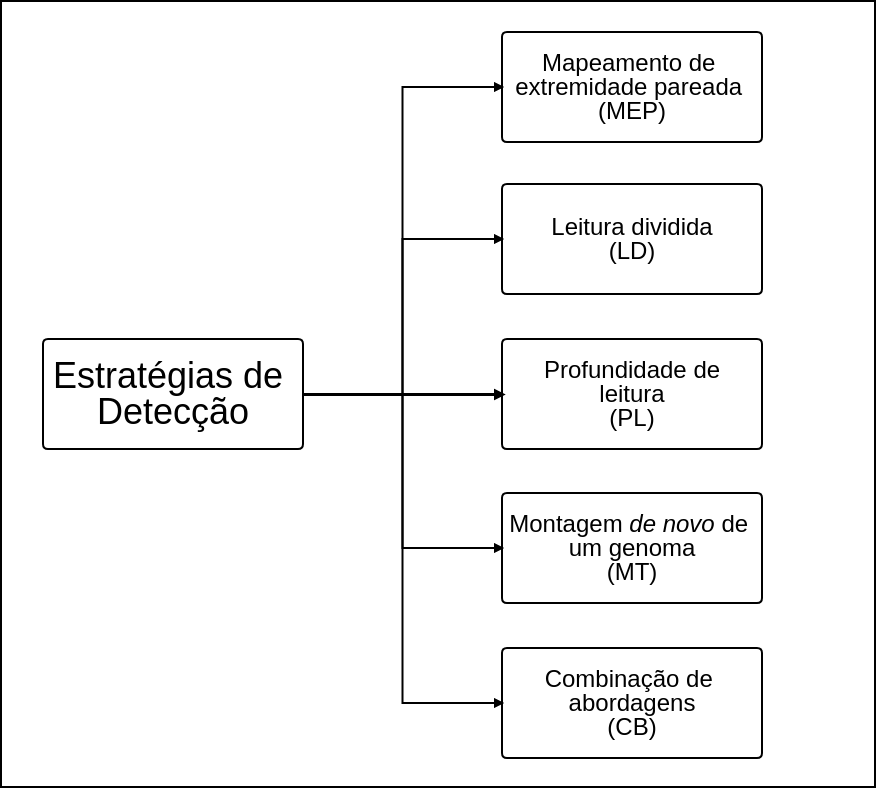
\includegraphics[width=0.8\textwidth]{./dados/figuras/estrategias-deteccao-cnv}
    \fonte{Autoria Própria}
    \label{fig:estrategias-deteccao-cnv}
\end{figure}

As abordagens da \autoref{fig:estrategias-deteccao-cnv} apresenta vantagens e limitações de acordo com o cenário a ser aplicado, sendo algumas das vantagens como no MEP em utilizações em leituras de final emparelhadas, ou em ferramentas que utilizam a abordagem LD, onde apresenta um maior desempenho em leituras curtas, mas independente disso, nenhuma das cinco abordagens é capaz de detectar todas as CNVs existentes \cite{Zhao2013}. 

O desenvolvimento de aplicações ligadas a essas estratégias se dá em linguagens de programação como R, C/C++, Java e outras. Apresentando diferentes abordagens para que a \textit{copy number variation} seja identificada e exposta, tentando alcançar uma maior performance \cite{Zhao2013}. 

\subsection{Métodos Avaliados} 

Nesta seção será apresentado a descrição alguns métodos focados na análise de \textit{copy number variation} que utilizam a estratégia de detecção baseada em profundidade em leitura (PL), ou seja, aplicações implementado modelos estatísticos focados em encontrar pontos de mudanças em uma série temporal, para alcançar o objetivo de encontrar a variação em dados do cromossomo \cite{Zhao2013}. A maioria das ferramentas descritas a seguir possuem natureza \textit{opensource}, assim sendo possível a contribuição da comunidade para o seu crescimento, com essa característica em mente, a evolução do mesmo pode ocorrer apos a publicação deste estudo, alterando a versão listada na \autoref{qua:ferramentas-de-deteccao-de-cnv}.


% Detecção
A detecção de CNVs passou por tecnologias como cariotipagem e hibridização fluorescente in situ (FISH) no início de pesquisas relacionadas ao tema, apos a descoberta da estrutura genômica completa, a detecção se deu por meio de hibridização genômica comparativa baseada em array (aCGH). O NGS possibilitou a melhoria na leitura de variações no número de cópias, obtendo uma maior performance ao ler os identificar as regiões variantes \cite{Zhao2013}. 

O método de identificação de CNV aplicado a dados gerados com ferramentas do NGS baseado em PL é utilizado para estimar o número de cópias, determinando sua localidade de acordo com as posições existente do cromossomo de amostra. A descoberta de CNVs segue quatro passos ao utilizar essa abordagem: mapeamento, normalização, estimativa do número de cópias e segmentação \cite{Zhao2013}.

A estimação do número de cópias pode ser resolvida de forma a aplicar algoritmos nos dados da amostra, como pode ser visto em algumas ferramentas existentes de detecção de CNV presentes no \autoref{qua:ferramentas-de-deteccao-de-cnv}. Esses modelos assumem a existência de perdas ou ganhos ao longo do cromossomo, aplicando algoritmos de distribuição de probabilidade na média e ou variância, a fim de detectar a localização de alguma variação no número de cópias \cite{Zhao2013}.


% ##### define colors
\definecolor{color000000}{RGB}{0,0,0}
% ##### FIM define colors

% ######## init table ########
\begin{table}[h]
 \centering
% distancia entre a linha e o texto
 {\renewcommand\arraystretch{1.25}
 \caption{Ferramentas de detecção de CNVs usando a abordagem de profundidade em leitura\label{qua:ferramentas-de-deteccao-de-cnv}}
 \begin{adjustbox}{max width=\textwidth}
\begin{tabular}{ l l l l l }
  \cline{1-1}\cline{2-2}\cline{3-3}\cline{4-4}\cline{5-5}  
    \multicolumn{1}{|c|}{\textbf{\textcolor{color000000}{Ferramenta}}} &
    \multicolumn{1}{c|}{\textbf{\textcolor{color000000}{Versão}}} &
    \multicolumn{1}{c|}{\textbf{\textcolor{color000000}{Linguagem}}} &
    \multicolumn{1}{c|}{\textbf{\textcolor{color000000}{Método}}} &
    \multicolumn{1}{c|}{\textbf{Referência}}
  \\  
  \cline{1-1}\cline{2-2}\cline{3-3}\cline{4-4}\cline{5-5}  
    \multicolumn{1}{|c|}{DNAcopy} &
    \multicolumn{1}{c|}{1.58.0} &
    \multicolumn{1}{c|}{R} &
    \multicolumn{1}{c|}{Segmentação binária circular (CBS)} &
    \multicolumn{1}{c|}{\cite{Olshen2004}}
  \\  
  \cline{1-1}\cline{2-2}\cline{3-3}\cline{4-4}\cline{5-5}  
    \multicolumn{1}{|c|}{fastseg} &
    \multicolumn{1}{c|}{1.30.0} &
    \multicolumn{1}{c|}{R} &
    \multicolumn{1}{c|}{Estrutura Bayesiana} &
    \multicolumn{1}{c|}{\cite{Baldi2001}}
  \\  
  \cline{1-1}\cline{2-2}\cline{3-3}\cline{4-4}\cline{5-5}  
    \multicolumn{1}{|c|}{iSeg} &
    \multicolumn{1}{c|}{1.3.2} &
    \multicolumn{1}{c|}{C++} &
    \multicolumn{1}{c|}{\textit{T-}testes simples para calcular \textit{p-}valores} &
    \multicolumn{1}{c|}{\cite{Girimurugan2018}}
  \\  
  \cline{1-1}\cline{2-2}\cline{3-3}\cline{4-4}\cline{5-5}  
    \multicolumn{1}{|c|}{CGHSeg} &
    \multicolumn{1}{c|}{1.0.2} &
    \multicolumn{1}{c|}{R} &
    \multicolumn{1}{c|}{Modelos lineares misto} &
    \multicolumn{1}{c|}{\cite{Picard2011}}
  \\
  \cline{1-1}\cline{2-2}\cline{3-3}\cline{4-4}\cline{5-5}  
    \multicolumn{1}{|c|}{ExomeDepth} &
    \multicolumn{1}{c|}{1.1.10} &
    \multicolumn{1}{c|}{R} &
    \multicolumn{1}{c|}{Modelo beta-binomial para ajuste de profundidade} &
    \multicolumn{1}{c|}{\cite{Plagnol2012}}
  \\ 
  \hline

 \end{tabular}
 \end{adjustbox}}
\end{table}

Os projetos apresentados no \autoref{qua:ferramentas-de-deteccao-de-cnv} possui suas peculiaridades de acordo com o método utilizado para identificação de CNVs, sendo alguns deles adaptados especificamente para a sua análise, como nos algoritmos implementados no DNAcopy, fastseg, CGHSeg, ExomeDepth. O iSeg é o único listado que se difere das ferramentas citadas acima, oferecendo uma análise genômica que abrange variação do número de cópias de DNA, ocupação do nucleossomo, sensibilidade à nuclease e dados de sensibilidade diferencial à nuclease \cite{Girimurugan2018}. 

\section{CHANGE POINT DETECTION}
\label{sec:changePointDetection}

% Introdução ao assunto CPD 
O estudo de dados coletados e distribuídos ao longo de um determinado tempo, também denominado como um série temporal (Time Serie/TS), é uma ferramenta muito utilizada para a observação, previsão e aprendizado de padrões em diversas áreas da ciência. Um problema recorrente ao analisar TS é a identificação de um ponto de variação que não era esperado no decorrer dos dados transcritos no gráfico, esse efeito é denominado como \textit{Change Point Detection} (Detecção de Ponto de Mudança/CPD) \cite{Aminikhanghahi2017}.

\begin{figure}[!htb]
    \centering
    \caption{Exemplo de série temporal com pontos de mudança}
    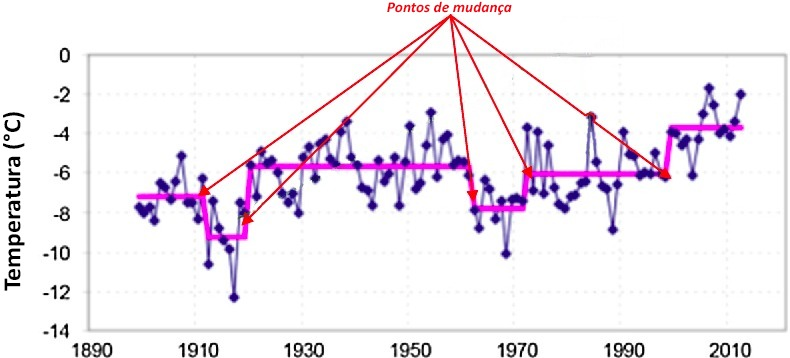
\includegraphics[width=0.8\textwidth]{./dados/figuras/pontos-de-mudanca}
    \fonte{Adaptado de \cite{Aminikhanghahi2017}}
    \label{fig:change-point}
\end{figure}

% Imagem e explicação de CPD de acordo com ela 
Ao observar a \autoref{fig:change-point}, é possível perceber que os elementos da série não permanecem em um único formato, variando em alguns pontos quando há alguma interferência no comportamento do componente percebido. A identificação das setas em vermelho exibe os pontos de mudança e as linhas horizontais na cor rosa são caracterizadas pelos estados normais da série temporal. A observação de pontos de mudanças em uma coleção de dados (\textit{dataset}) com muitos variantes, muitas vezes necessita da utilização de algoritmos, a fim de obter uma maior precisão na detecção. 

A aplicação de desse conceito tem sido bastante explorada em vários cenários na atualidade, como em análises de imagem, reconhecimento de padrões, biomédico \cite{Fan2015}, \textit{cybersecurity} \cite{Polunchenko2012}, séries climáticas \cite{Bates2012}, entre outros. 

Os objetivos fixados ao estudar pontos de mudança geralmente estão entre saber se existe alguma variação, e se existir saber se é mais de uma e quais os seus respectivos locais em um determinado tempo \cite{Chen1-2000}.

\subsection{Formulação do Problema}

Seja $X_1, X_2, ..., X_n$ uma sequência de vetores aleatórios independentes (variáveis) com funções de distribuição de probabilidade $F_1, F_2, ..., F_n$, respectivamente. Então, o problema de \textit{change point} é testar a seguinte hipótese nula:

\begin{equation}
    H_0 : F_1 = F_2 = ... = F_n
    \label{eq:cpd-hupotese-nula-1}
\end{equation}

versus a hipótese alternativa

\begin{equation}
    H_{1} : F_{1} = ... = F_{k_1}\neq F_{{k_1}+1} = ... = F_{k_2}\neq F_{{k_2}+1} = ... F_{k_q}\neq F_{{k_q}+1} ... = F_{n},
    \label{eq:cpd-hipotese-alternativa-1}
\end{equation}

onde $1 < k_1 < k_2 < ... < k_q <n$, $q$ é o número desconhecido de pontos de mudança e $k_1, k_2, ..., k_q$ são as respectivas posições que devem ser estimadas. Se as distribuições $F_1, F_2, ..., F_n$ pertencem a uma família paramétrica comum $F(\theta)$, 
então o problema do ponto de mudança é testar hipóteses sobre os parâmetros da população $\theta_i$, com a sequência $i = 1 ..... n$

\begin{equation}
    H_0 : \theta_{1} = \theta_{2} = ... = \theta_{n} = \theta (desconhecido)
    \label{eq:cpd-hupotese-nula-2}
\end{equation}

versus a alternativa

\begin{equation}
    H_1 : \theta_{1} = ... = \theta_{k_1} \not = \theta_{{k_1}+1} = ... = \theta_{2} \not = ... \not = \theta_{{k_q}-1} = ... = \theta_{k_q} \not = \theta_{{k_q}+1}... = \theta_{n},
    \label{eq:cpd-hipotese-alternativa-2}
\end{equation}

onde $q$ e $k_1, k_2, ..., k_q$ precisam ser estimados. Essas hipóteses combinadas revelam aspectos da inferência de ponto de mudança, ou seja, os objetivos citados acima. 

As hipóteses apresentadas se adéquam a problemas relacionado a busca de um simples ponto de mudança, entretanto ela pode ser adaptada para aderirem problemas de múltiplos pontos de mudança em uma coleção de dados \cite{Chen1-2000}. 

\subsection{Tipos de Pontos de Mudança} 

Os pontos de mudança podem ser observados a partir de uma representação gráfica das distribuições dos valores de uma coleção. Contudo, as mudanças ocorridas podem ser classificadas de acordo com o tipo de mudança, seja ela, mudança na média, na variância, em ambos simultaneamente, além de vários tipos de modelos propostos ao longo do tempo \cite{Chen2-2000}. 

A aplicação desses modelos de ponto de mudança é apresentada por diversos autores, assim como em \cite{Cheon2010} ao apresentar um a utilização da detecção por média em um modelo Bayesian e no \cite{Shi2017} ao descrever a utilização de um modelo baseado em grafos para análise de modelos de grande dimensão. 


% A detecção de pontos de mudança pode ser classificada de duas formas, Online e Offline, onde a forma online é um processamento de dados ao vivo, tentando detectar o ponto antes que ocorra realmente. O método de detecção offline possui uma maior flexibilidade em relação ao online, sendo capaz de analisar toda a série disponível para realizar as identificadões necessárias \cite{Aminikhanghahi2017}.
% Abordar as formas que são utilizadas para identificar


% Ligar CPD ao CNV
% A CPD é explorada em diversos campos de estudo por ser um tópico relevante no observação de uma coleção, com o surgimento do NGS houve um grande aumento em pesquisas relacionadas a análise de ponto de mudança focados em CNV, impulsionando o desenvolvimento de aplicações que usam os algoritmos propostos na formulação de \textit{Change Point Detection} \cite{Xi2011}.

\subsection{Algoritmos Relacionados}

Nesta seção será apresentado algoritmos desenvolvidos com o proposito de segmentar \textit{datasets} e determinar pontos de mudanças caso haja. Os algoritmos apresentados possuem características de determinação de \textit{change point} divergentes, ou seja, cada um deles possuem uma abordagem própria para a segmentação dos dados \cite{Aminikhanghahi2017}. A seguir encontra-se a definição de algumas ferramentas disponíveis para utilização gratuita (\textit{open source}):

\subsubsection{CBS}

O CBS (Circular Binary Segmentation) é uma modificação de uma estratégia de segmentação binária, proposta com a finalidade de segmentar o cromossomo, apresentando funcionalidades adicionais para normalizar os dados. A segmentação binária é uma técnica aplicada para a determinar a localização de um ponto de mudanças com a aplicação de testes recursivos \cite{Olshen2004}.

Um dos objetivo na proposta do CBS foi a identificação de segmentos menores dentro de segmento maiores de mudanças. Devido a níveis de significância pequenos aplicados aos cálculos uma grande quantidade de permutações é realizada na determinação de somente um ponto de mudança, chegando a ordem de dez mil, esse processo é feito para cada segmento existente na coleção de dados \cite{Olshen2004}.

Devido ao custo computacional do cálculo em dados grande ser alto em sua época de desenvolvimento, os dados são repartidos em janelas sobrepostas com tamanhos aproximadamente iguais, para alcançar uma maior performance ao procurar ponto de mudanças \cite{Olshen2004}.

O CBS mostrou ter um desempenho consistente, diante de comparações com técnicas semelhantes, onde se destacou por sua pela sensibilidade na detecção e a taxa de falsos negativos \cite{Hsu2011}.

% \subsubsection{ecp}

\subsubsection{gSeg}

O gSeg (Graph Segmentation) é um algoritmo baseado em grafos, para a detecção de pontos de mudanças de acordo com o agrupamento de observações próximas das distâncias representadas por grafos, onde será identificado a similaridade entre os pontos, para determinação de uma variação 
\cite{Chen2015}. 

A sua execução é dada pela divisão de dois grupos, sendo eles o grupo que vem antes de $\tau$ e o grupo que vem depois de $\tau$, onde cada grupo um número mínimo de observações correspondente a $1 < n_{0} \leq \tau \leq n_{1} < n$ em um único cenário de ponto de mudança, podendo ser adicionado restrições de acordo com o modelo analisado. A partir da divisão, é realizado um teste de grafo, a fim de verificar se os grupos possuem distribuições similares \cite{Chen2015}. 

O método de detecção baseado em grafos é recomendado para testes em dimensões moderadas e altas, exigindo poucas informações acerca delas para realizar a varredura responsável pela segmentação em grafos. Testes técnicas de varredura diferentes foram testados, a fim ver o seu progresso de acordo com os dados de entrada, obtendo resultados abaixo da média em somente uma das técnicas \cite{Chen2015}. 

O gSeg segue o viés de detecção de um ponto de mudança, mas de acordo com \cite{Chen2015}, o método de segmentação por grafos pode ser aplicado recursivamente ao procedimento do \textit{Circular Binary Segmentation}, se haver a necessidade de aplica-lo em cenários que apresenta mais de um ponto de mudança.


\subsubsection{PELT}

O \textit{Pruned Exact Linear Time} (PELT) descrito no \autoref{alg:pelt} foi proposto por \cite{Killick2012}, a sua base de desenvolvimento está no algoritmo \textit{Optimal Partitioning} (OP) descrito por \cite{Gioumousis2005} de forma a melhorar o desempenho obtido por seu antecessor. 

Em \autoref{alg:op} podemos ver um pseudocodigo que representa o algoritmo OP. A principal diferença entre os dois algoritmos citados acima é a redução de visualização de \textit{change points} anteriores ao calculado encontrado na proposta do método PELT onde somente alguns pontos de mudança são percorridos \cite{BenedicteBakka2018}. 

\begin{algorithm}
    \caption{Optimal Partitioning Algorithm (OP).\label{alg:op}}
    \KwIn{
    Um conjunto de dados $(y1, y2, ..., yn)$ denominado como $Y$.\\
    Uma constante de penalidade denominada \beta.\\
    Uma função de custo $C(.)$ para medir o ajuste dependendo dos dados.
    }
    \KwOut{Vetor de pontos de mudança encontrados $\tau = (\tau_1, ..., \tau_m, \tau_m_+_1)$}
    \Begin{
        Inicialização: 
        $n = length(Y)$\\
        $F(0) = -$\beta\\
        \For{$t\leftarrow 1$ \KwTo $n$} {
            $F(t) =$ \infty\\
            \tcc{Pecorre todo o conjunto de dados para cada ponto $y_t$ para encontrar o melhor ponto de mudança anterior $y_s$ }
            \For{$s \leftarrow 0$ \KwTo $t-1$}{
                \tcc{Calcular o custo total esperado de $t$ de acordo com $s$}
                $p = F(s)+C(s +1,t)+\beta$\\
                \tcc{Se a redução feita for por meio do s}
                \If{$p < F(t)$}{
                    \tcc{Registrar nova estimativa para $F(t)$}
                    $F(t) = p$\\
                    \tcc{Registrar o melhor ponto de mudança anterior em $t$ igual a $s$}
                    $r(t) = s$
                }
            }
        }
        \tcc{Contruir um vetor $\tau$ de $r$}
        $changepoint = n$\\
        $i = 1$\\
        \While {changepoint \not= 0} {
            $\tau(i) = changepoint$\\
            $changepoint =r (changepoint)$\\
            $i = i + 1$
        }
        \tcc{Inverter o vetor $\tau$ para obtemos a sequencia correta $(\tau_1, ..., \tau_m, \tau_m_+_1)$}
        $\tau = Sort(\tau)$
    }
\end{algorithm}
 
\begin{algorithm}
    \caption{Pruned Exact Linear Time (PELT).\label{alg:pelt}}
    \KwIn{
    Um conjunto de dados $(y1, y2, ..., yn)$ denominado como $Y$.\\
    Uma constante de penalidade denominada \beta.\\
    Uma função de custo $C(.)$ para medir o ajuste dependendo dos dados.\\
    Uma constante K.
    }
    \KwOut{Vetor de pontos de mudança encontrados $\tau = (\tau_1, ..., \tau_m, \tau_m_+_1)$}
    \Begin{
        Inicialização: 
        $n = length(Y)$\\
        $F(0) = -$\beta\\
        $s.set = {0}$\\
        \For{$t\leftarrow 1$ \KwTo $n$} {
            $F(t) =$ \infty\\
            \tcc{Calcular o custo total esperado de $t$ de acordo com $s$}
            \For{$s \in s.set$} {
                $p = F(s)+C(s +1,t)+\beta$\\
                \tcc{Se a redução feita for por meio do s}
                \If{$p < F(t)$}{
                    \tcc{Registrar nova estimativa para $F(t)$}
                    $F(t) = p$\\
                    \tcc{Registrar o melhor ponto de mudança anterior em $t$ igual a $s$}
                    $r(t) = s$
                }
            }
        }
        \For{$s \in s.set$}{
            \If{$F(s)+C(s +1,t)≥F(t)$}{
                $Remove(s.set, s)$
            }
        }
        $Append(s.set,t)$\\
        \tcc{Contruir um vetor $\tau$ de $r$}
        $changepoint = n$\\
        $i = 1$\\
        \While {changepoint \not= 0} {
            $\tau(i) = changepoint$\\
            $changepoint =r (changepoint)$\\
            $i = i + 1$
        }
        \tcc{Inverter o vetor $\tau$ para obtemos a sequencia correta $(\tau_1, ..., \tau_m, \tau_m_+_1)$}
        $\tau = Sort(\tau)$
    }
\end{algorithm}


A diferença entre as descrições dos algoritmos propostos pode ser vista a partir da segunda linha de do laço de repetição for, apresentando uma interação diferente se comparar o mesmo ponto em ambos algoritmos. Essa diferença se da por causa da proposta de do método PELT, visando aumentar a eficiência computacional, fazendo com que valores inválidos sejam excluídos em uma minimização \cite{Killick2012}. 

Ao realizar a minimização, assumimos que existe uma constante $K$ tal que, para todo $t < s < T$, onde t nunca poderá ser o melhor ponto de mudança antes de T. 

\begin{equation}
    C\left ( y\left ( t+1 \right ):s \right ) + C\left ( y\left ( t+1 \right ):T \right ) + K \leq C\left ( y\left ( t+1 \right ):T \right )
    \label{eq:calculo-pelt}
\end{equation}


\subsubsection{SpecDetec}

O algoritmo de espectro de grafos (\textit{Graph Spectrum}) proposto por \cite{Uzai2019} é uma adaptação do gSEG, onde apresenta como atividade principal a análise de valores estatísticos de varreduras com grafos, agrupando dados que estão conectados. 

O espectro de grafos é a representação dos autovalores, ou seja, valores contidos na diagonal de uma matriz de um grafo determinado $G$, esses autovalores podem ser vistos na matriz de adjacência calculada a partir do grafo, de tal forma que $A(G)$ \cite{Uzai2019}. 

O funcionamento do algoritmo é determinado pelos passos de determinação de uma matriz de similaridade entre pontos $x$ e $y$, assim obtendo $S_{ij} = (x_{i}, y_{j})$.A partir do calculo da matriz $S$ com a medida de similaridade Gaussiana é obtido uma matriz de afinidade, usada para o repartimento entre si obtendo \textit{clusters}, assim podendo ser identificados os pontos de mudança \cite{Uzai2019}.

A análise de resultados em comparação com algoritmos que possuem o mesmo objetivo, mas com técnicas para alcança-lo diferentes entre si, alcançou valores satisfatórios ultrapassando os algoritmos SegNeigh, PELT e EDivisive. A análise de espectro de grafos obteve somente resultada abaixo dos outros métodos comparados em uma base de dados, onde os demais algoritmos obtiveram uma baixa nos seus resultados também \cite{Uzai2019}.

\subsubsection{TSMCP}

O algoritmo TSMCP, abreviação de \textit{Fast Two Stage Multiple Change Point Detection}, baseado no laço adaptativo proposto por \cite{Zou2006}, onde utiliza-se pesos adaptativo para penalizar os coeficientes a fim de selecionar as variáveis. O método proposto contém estágios de corte e refinamento para estimar simultaneamente múltiplos pontos de mudança em modelos lineares \cite{Jin2016}. 

O procedimento da composição das etapas de estimação dos números de pontos de mudanças e suas respectivas localizações, essa técnica apresentou um maior desempenho em coleções de dados menores, pela quantidade de repetições a ser realizada na etapa de corte \cite{Jin2016}. 

A fase de corte, é onde será sequenciado o conjunto de dados e a partir dele é suposto a existência de um ponto de mudança nesse segmento, como o modelo visto utiliza de regressão linear, é feita uma regularização de com os mínimos quadrados para obter estimadores iniciais, utilizados para determinação dos pontos de mudança \cite{Jin2016}. 

A fase de refino é responsável pela verificação da existência de alguma variação dentro das áreas obtidas na fase de corte, para alcançar esse objetivo é aplicado um teste de razão de quase verossimilhança em cada segmento gerado afim de estimativas de pontos de mudanças \cite{Jin2016}.

\section{MATRIZ DE CONFUSÃO}
\label{sec:matrizDeConfusao}

A matriz de confusão é uma forma de validar experimentos, sua utilização se dá em cenários de análise de resultados provenientes de experimentos desenvolvidos. Com a aplicação desta técnica, resultados como frequência de acertos e erros em relação ao resultado esperado no experimento podem observados e investigados para assim melhorar o rendimento encontrado na análise \cite{Ruuska2018}.

\begin{figure}[!htb]
    \centering
    \caption{Exemplo de matriz de confusão}
    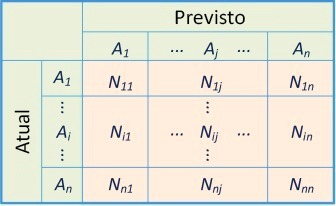
\includegraphics[width=0.6\textwidth]{./dados/figuras/matriz-de-confusao}
    \fonte{Adaptado de \cite{Deng2016}}
    \label{fig:matriz-confusao}
\end{figure}

Uma matriz de confusão é composta por duas dimensões, sendo elas os valores reais e os valores previstos, onde eventualmente eles serão usados para obter uma classificação do método avaliado de acordo com o seu desempenho \cite{Deng2016}. Existe demasiados modelos para se obter os valores da performance do objeto estudado, sendo as medidas mais comuns apresentadas a segui.

\begin{itemize}
   \item Acurácia (AC):
   \begin{description}
    \item Medida usada para calcular o total de previsões corretas dentro dos resultados obtidos
    \begin{equation}
        AC=\sum_{i=1}^nN_{ii}/\sum_{i=1}^n\sum_{j=1}^nN_{ij}
    \label{eq:mc-acuracia}
    \end{equation}
    \end{description}
    \item Precisão (PC):
    \begin{description}
    \item Medida usada para saber a exatidão obtida por determinada classe analisada
    \begin{equation}
        PC_i=N_{ii}/\sum_{k=1}^nN_{ki}
    \label{eq:mc-precisao}
    \end{equation}
    \end{description}
    \item Sensibilidade (SB):
    \begin{description}
    \item Medida usada para saber a probabilidade de acerto de uma determinada classe
    \begin{equation}
        SB_i=N_{ii}/\sum_{k=1}^nN_{ik}
        \label{eq:mc-sensibilidade}
    \end{equation}
    \end{description}
    \item F-Score (Fscore):
    \begin{description}
    \item Medida usada para obter a média harmônica entre a precisão e a sensibilidade
    \begin{equation}
        Fscore_i=\frac{2\times PC_i\times SB_i}{PC_i+SB_i}
        \label{eq:mc-fscore}
    \end{equation}
    \end{description}
\end{itemize}         % Revisão de Literatura
% METODOLOGIA------------------------------------------------------------------

\chapter{METODOLOGIA}
\label{chap:metodologia}
Esse capítulo abordará a forma de desenvolvimento de uma ferramenta focado na análise de \textit{copy number variation} a partir de algoritmos especializados na detecção de \textit{change point}, além de ser apresentado os dados de testes, as tecnologias e o recurso de validação a ser utilizados no método proposto.

\section{MÉTODO PROPOSTO}

A proposta desse trabalho está focada na utilização dos conceitos de CPD no contexto de captura de CNV, para que assim seja desenvolvido uma ferramenta de segmentação de dados do exoma capaz de utilizar mais de um método de detecção de ponto de mudança. A estrutura dessa ferramenta deverá ser capaz de executar a leitura de dados de exoma, disponibilizando formas de escolher um método de segmentação de CPD e de retornar os dados segmentados apresentando informações relevantes sobre os dados analisado, como a existência de alguma variação no número de cópias.

O projeto será construído utilizando a Linguagem R, para facilitar a utilização e integração de projetos existentes que detectam pontos de mudanças. Ele se baseará na estruturação do DNAcopy \cite{Olshen2004} para o desenvolvimento da leitura e segmentação dos dados.

\section{TECNOLOGIAS UTILIZADAS}

Nesta seção são descritas as tecnologias utilizadas para o desenvolvimento do projeto, apresentando uma breve contextualização e definindo conceitos essenciais para o entendimento do ambiente de criação da pesquisa.

\subsection{R Project}

O R \cite{Core2019} é uma linguagem e um ambiente focado em computação estatística e gráficos, contendo um módulo complementar incluso ao seu ambiente com vários pacotes de procedimentos estatísticos, apresentação de dados gráficos e outros disponibilizados para o uso nos mais diversos contextos \cite{website:Hornik2018}.

O R permite a criação de \textit{scripts} de execução, desde contas matemáticas simples como uma soma, até a execução de algoritmos complexos e/ou exibição de gráficos sobre determinados dados. A plataforma permite o agrupamento de variados \textit{scripts} em subdiretórios (pasta de trabalho) para obter uma maior organização ao nível de código, possibilitar os testes, a documentação e a distribuição dos códigos criados, o conjunto de todos os arquivos referentes a essa estrutura é denominada como pacote \cite{website:Hornik2018}.

\subsubsection{PACOTES R}

O pacote R é uma forma de agrupar um código em um padrão de projeto para que seja mais fácil a distribuição e a utilização por terceiros, a disponibilização da maioria dos pacotes R é contida na plataforma CRAN \cite{website:Hornik2018}.

O \autoref{qua:ferramentas-cpd} apresenta alguns pacotes R relacionados ao tema de detecção de pontos de mudanças. Esses pacotes implementam estrategias de detecção baseadas em algoritmos capazes de identificar e localizar um ou mais pontos de mudança em uma coleção de dados disponibilizada pelo usuário.

\begin{quadro}[hbp]
\centering
\caption{Pacotes R de algoritmos de detecção de pontos de mudança \label{qua:ferramtas-cpd}}
    \begin{adjustbox}{max width=\textwidth}
    \begin{tabular}{ | c | c | p{5cm} | p{5cm} | } \hline
        \textbf{Nome}     & \textbf{Versão}      & \textbf{Algoritmo}     & \textbf{Referência} \\ \hline
        bcp & 4.0.3 &  & \cite{Emerson2007} \\ \hline
        breakfast & 1.1.1 &  & \cite{Fryzlewicz2017} \\ \hline
        changepoint & 2.2.2 &  & \cite{Eckley2016} \\ \hline
        SpecDetec & 1.0.0 &  & \cite{Uzai2018} \\ \hline
    \end{tabular}
    \end{adjustbox}
\end{quadro}

\subsubsection{CRAN}

O \textit{Comprehensive R Archive Network} (CRAN) é uma plataforma para o arquivamento de pacotes R, para facilitar o acesso a versões e informações críticas de um pacote, como a documentação e as instruções de instalação. A partir dele é possível a obtenção de binários pré-construídos para vários sistemas operacionais (Linux, Mac OS Classic, macOS e MS Windows), arquivos zipados e outros. Os pacotes distribuídos pelo CRAN estão disposto a comunidade para utilização e contribuição, devido a sua natureza \textit{open source} \cite{website:Hornik2018}.

\subsection{GitHub}

O GitHub \cite{GitHub2019} é uma plataforma de hospedagem de código-fonte versionado pelo Git\footnote{Sistema de controle de versões de projetos, capaz de registrar o histórico de edições}, ele dispõe de funcionalidades do Git em interface gráfica e acrescenta recursos necessários para a colaboração em repositórios públicos e privados, além de oferecer ferramentas e extensões para o controle de projetos. O GitHub amplamente utilizada e já chegou a registrar três milhões de projetos mantidos por mais de um milhão de desenvolvedores registrados \cite{Thung2013}.

\section{DESENVOLVIMENTO}

\subsection{Visão Geral}

A construção do projeto proposto será implantada na linguagem R, seguindo os padrões sugeridos ao criar um pacote para que a distribuição dele possa ser feita pelo CRAN. O código-fonte e documentação produzida serão armazenadas de forma \textit{open source} nas plataformas do GitHub e CRAN, facilitando o controle de versão e a contribuições futuras ao projeto.

Para a criação do projeto será usado como base algumas das ferramentas especificas para busca de CNVs e CPD, se baseando na estrutura delas para formulação de um ambiente especializado em leituras de dados sequenciado do exoma. Uma das principais fonte de dados na qual o projeto se baseará será o DNAcopy, retirando ideias e conceitos semelhantes.

A segmentação dos dados será dada pela integração de pacotes de detecção de ponto de mudanças contidos no CRAN, adaptando-os se necessário para que eles possam identificar as variações do exoma.

\subsubsection{Fluxo de Funcionamento}

O modelo de processo de funcionamento descrito na \autoref{fig:metodologia-tcc}, terá 2 etapas de responsabilidade do usuário, sendo elas entrada de dados e as configurações iniciais. A partir da inserção das informações pedidas ao usuário, o algoritmo será capaz de realizar o processamento das informações inseridas em 4 etapas de execução, preparação dos dados, aplicação da segmentação, identificação dos pontos de mudança e a organização dos resultados e informações inseridas.

\begin{figure}[!htb]
    \centering
    \caption{Representação gráfica do processo de detecção de pontos de mudança com múltiplos algoritmos de segmentação}
    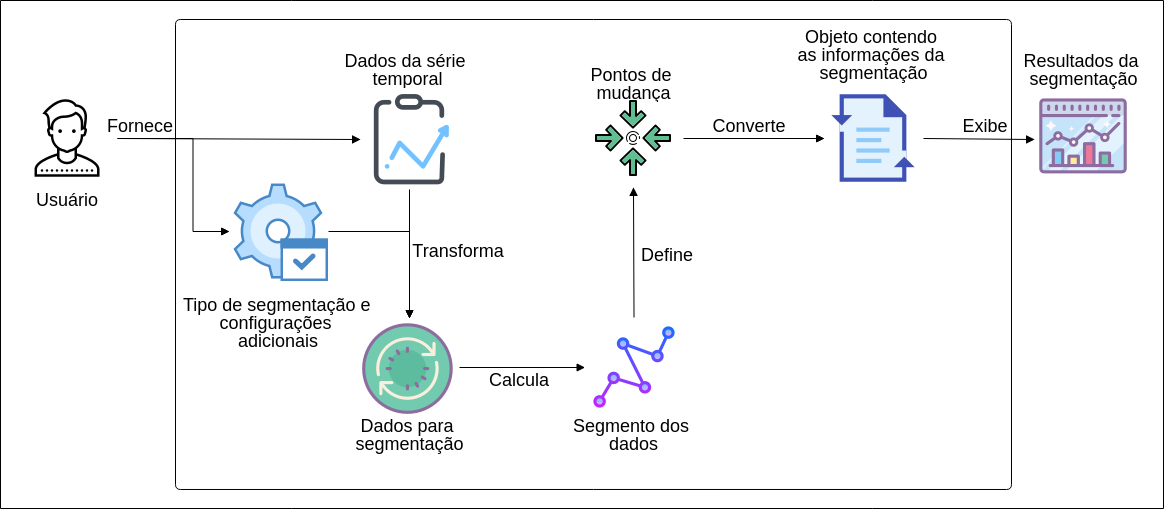
\includegraphics[width=1\textwidth]{./dados/figuras/metodologia-tcc}
    \fonte{Autoria Própria}
    \label{fig:metodologia-tcc}
\end{figure}

Os métodos de segmentação de entrada poderá ser escolhidos através de parâmetros na função de segmentação, assim podendo ser identificado qual método escolhido e quais atributos adicionais serão inseridos referente ao modelo de segmentação selecionado.

A partir da segmentação, a saída dos resultados irá ser padronizada com os dados de entrada, os resultados dos cálculos e informações referentes a chamada da função, descrevendo quais os parâmetros utilizados no cálculo dos pontos de mudança. Portanto, com o objeto retornado será possível plotar gráficos de acordo com o desejo do usuário, ao usar as funções de plotar da linguagem R.

\section{BASE DE DADOS} 
\label{sec:baseDeDados} 

Com o objetivo de testar o desempenho e funcionamento do algoritmo criado, os dados do Coriell \cite{Snijders2001} será utilizado, utilizando as linhas celulares disponibilizadas pelo projeto. Esses dados são utilizados em vários projetos similares, como o DNAcopy \cite{Olshen2004} e \cite{Girimurugan2018}. Entretanto, caso haja a necessidade, será retirada informação de outros sequenciamentos do GenBank\footnote{Acesso ao site através do seguinte endereço https://www.ncbi.nlm.nih.gov/genbank/} e outras fontes que disponibilizem os dados de forma gratuitas.

Os dados disponibilizados como Coriell possui informações relevantes sobre a linha celular, como o clone que as informações foram tiradas, o cromossomo de referência, a sua variação e assim por diante. A estrutura presente nas informações disponibilizadas do coriell contem elementos como a \autoref{tab:tabela-2-dados}, onde são apresentadas os cinco primeiros elementos referente a linha celular do GM05296 e GM13330, dispostas pelo Coriell \cite{Snijders2001}.

% ######## init table ########
\begin{table}[h]
 \centering
% distancia entre a linha e o texto
 {\renewcommand\arraystretch{1.25}
 \caption{Cinco primeiros dados do Coriell correspondentes a amostra GM05296 e GM13330 contidos na base do DNAcopy}
 \label{tab:tabela-2-dados}
 \begin{tabular}{ l l l l l }
  \cline{1-1}\cline{2-2}\cline{3-3}\cline{4-4}\cline{5-5}  
    \multicolumn{1}{c}{Clone \centering } &
    \multicolumn{1}{c}{Chromosome \centering } &
    \multicolumn{1}{c}{Position \centering } &
    \multicolumn{1}{c}{Coriell.05296 \centering } &
    \multicolumn{1}{c}{Coriell.13330 \centering }
  \\  
  \cline{1-1}\cline{2-2}\cline{3-3}\cline{4-4}\cline{5-5}  
    \multicolumn{1}{c}{GS1-232B23 \centering } &
    \multicolumn{1}{c}{1 \centering } &
    \multicolumn{1}{c}{0 \centering } &
    \multicolumn{1}{c}{NA \centering } &
    \multicolumn{1}{c}{0.207470 \centering }
  \\  
  \cline{1-1}\cline{2-2}\cline{3-3}\cline{4-4}\cline{5-5}  
    \multicolumn{1}{c}{RP11-82d16 \centering } &
    \multicolumn{1}{c}{1 \centering } &
    \multicolumn{1}{c}{468 \centering } &
    \multicolumn{1}{c}{0.008824 \centering } &
    \multicolumn{1}{c}{0.063076 \centering }
  \\  
  \cline{1-1}\cline{2-2}\cline{3-3}\cline{4-4}\cline{5-5}  
    \multicolumn{1}{c}{RP11-62m23 \centering } &
    \multicolumn{1}{c}{1 \centering } &
    \multicolumn{1}{c}{2241 \centering } &
    \multicolumn{1}{c}{-0.000890 \centering } &
    \multicolumn{1}{c}{0.123881 \centering }
  \\  
  \cline{1-1}\cline{2-2}\cline{3-3}\cline{4-4}\cline{5-5}  
    \multicolumn{1}{c}{RP11-60j11 \centering } &
    \multicolumn{1}{c}{1 \centering } &
    \multicolumn{1}{c}{4504 \centering } &
    \multicolumn{1}{c}{0.075875 \centering } &
    \multicolumn{1}{c}{0.154343 \centering }
  \\  
  \cline{1-1}\cline{2-2}\cline{3-3}\cline{4-4}\cline{5-5}  
    \multicolumn{1}{c}{RP11-111O05 \centering } &
    \multicolumn{1}{c}{1 \centering } &
    \multicolumn{1}{c}{5440 \centering } &
    \multicolumn{1}{c}{0.017303 \centering } &
    \multicolumn{1}{c}{-0.043890 \centering }
  \\  
  \hline

 \end{tabular} }
 \fonte{Autoria Própria}
\end{table}

\section{VALIDAÇÃO} 

O trabalho proposto será validado para que haja uma garantia de que os pontos de mudanças sejam conservados no mesmo local, assim obtendo uma maior veracidade na confiança do trabalho desenvolvido. Portanto, para garantir efetividade do algoritmo criado será utilizada a Matriz de Confusão aplicada aos dados descritos na \autoref{sec:baseDeDados} para obter uma análise do desempenho do algoritmo.                   % Metodologia
% PLANO DE TRABALHO-------------------------------------------------------------------

\chapter{PLANO DE TRABALHO}
\label{chap:planoDeTrabalho}

Cada capítulo deve conter uma pequena introdução (tipicamente, um ou dois parágrafos) que deve deixar claro o objetivo e o que será discutido no capítulo, bem como a organização do capítulo.
Este capítulo será a descrito o cronograma 
 é apresentado o cronograma e as atividades desenvolvidas durante um determinado período para que a execução do projeto se conclua.

\section{CRONOGRAMA}

\begin{figure}[!htb]
    \centering
    \caption{Cronograma das atividades a serem realizadas no desenvolvimento do projeto}
    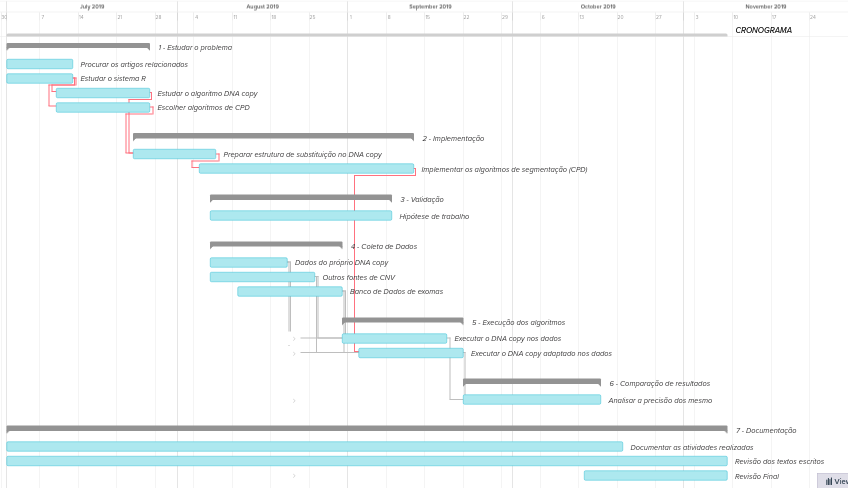
\includegraphics[width=1\textwidth]{./dados/figuras/cronograma}
    \fonte{Autoria Própria}
    \label{fig:cronograma}
\end{figure}

\subsection{Atividades do Cronograma}

O cronograma para o desenvolvimento do projeto apresenta um conjunto de sete grupos de atividades (\textit{milestones}) que representam o marco de histórico de cada uma das sub atividades que se encontram anhiadass nessa \textit{milestone}, como visto na \autoref{fig:cronograma}. A definição e levantamento desse grupos de atividades se deu ao analisar a necessidade dos requisitos e objetivos a serem atendidos para o desenvolvimento do projeto.

A seguir encontra-se uma descrição do maior grupo de atividades a serem executadas neste projeto:

\begin{enumerate}
   \item Estudar o problema
   \begin{description}
        \item[Início] 01/07/19
        \item[Fim] 26/07/19
        \item[Descrição] Investigação do assunto referente ao problema, buscando o entendimento de \textit{Change Point} e a aplicação de algoritmos de segmentação (CPD), \textit{Copy Number Variation}, linguagem R e a estrutura do DNAcopy.
    \end{description}
   \item Implementação
   \begin{description}
        \item[Início] 24/07/19
        \item[Fim] 12/09/19
        \item[Descrição] Desenvolvimento da estrutura para criação do projeto proposto, efetivando o objetivo proposto no trabalho, com a implementação da ferramenta para análise de CNV com vários algoritmos de CPD.
    \end{description}
   \item Validação
   \begin{description}
        \item[Início] 07/08/19
        \item[Fim] 08/09/19
        \item[Descrição] Definição da uma hipótese de trabalho e formulação da estrutura a fim de trabalhar com ela na atividade de comparação dos resultados, buscando definir a validação das funcionalidades do projeto, de acordo com a sua efetividade e desempenho.
    \end{description}
   \item Coleta de Dados
   \begin{description}
        \item[Início] 07/08/19
        \item[Fim] 30/08/19
        \item[Descrição] Busca por dados a serem utilizados como teste no projeto criado e em trabalhos de comparação com mesmo.
    \end{description}
   \item Execução dos algoritmos
   \begin{description}
        \item[Início] 31/08/19
        \item[Fim] 21/09/19
        \item[Descrição] Execução e coleta de dados gerados a partir dos testes realizados em trabalhos similares.
    \end{description}
   \item Comparação dos resultados
   \begin{description}
        \item[Início] 22/09/19
        \item[Fim] 16/10/19
        \item[Descrição] Análise dos dados da aplicação dos algoritmos testados de acordo com a Matriz de Confusão descrita na \autoref{sec:matrizDeConfusao}.
    \end{description}
   \item Documentação
   \begin{description}
        \item[Início] 01/07/19
        \item[Fim] 08/11/19
        \item[Descrição] Levantamento da escrita sobre as atividades realizadas e dados obtidos com o desenvolvimento do projeto.
    \end{description}
 \end{enumerate}          % Plano de Trabalho
% % RESULTADOS-------------------------------------------------------------------

\chapter{ANÁLISE E DISCUSSÃO DOS RESULTADOS}

Cada capítulo deve conter uma pequena introdução (tipicamente, um ou dois parágrafos) que deve deixar claro o objetivo e o que será discutido no capítulo, bem como a organização do capítulo.
                    % Resultados
% % ORIENTAÇÕES GERAIS------------------------------------------------------------


% SOBRE AS ILUSTRAÇÕES----------------------------------------------------------
\chapter{SOBRE AS ILUSTRAÇÕES}
\label{chap:apSobreIlust}

A seguir exemplifica-se como inserir ilustrações no corpo do trabalho. As ilustrações serão indexadas automaticamente em suas respectivas listas. A numeração sequencial de figuras, tabelas e equações também ocorre de modo automático.

Referências cruzadas são obtidas através dos comandos \verb|\label{}| e \verb|\ref{}|. Sendo assim, não é necessário por exemplo, saber que o número de certo capítulo é \ref{chap:fundamentacaoTeorica} para colocar o seu número no texto. Outra forma que pode ser utilizada é esta: \autoref{chap:fundamentacaoTeorica}, facilitando a inserção, remoção e manejo de elementos numerados no texto sem a necessidade de renumerar todos esses elementos.

% FIGURAS-----------------------------------------------------------------------
\chapter{FIGURAS}
\label{chap:figuras}

Exemplo de como inserir uma figura. A \autoref{fig:figura-exemplo1} aparece automaticamente na lista de figuras. Para saber mais sobre o uso de imagens no \LaTeX{} consulte literatura especializada \cite{Goossens2007}.

Os arquivos das figuras devem ser armazenados no diretório de "/dados".

\begin{figure}[!htb]
    \centering
    \caption{Exemplo de Figura}
    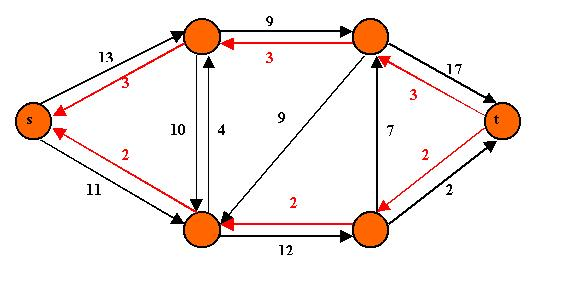
\includegraphics[width=0.5\textwidth]{./dados/figuras/figura1}
    \fonte{\citeonline{IRL2014}}
    \label{fig:figura-exemplo1}
\end{figure}

% QUADROS E TABELAS---------------------------------------------------------------
\chapter{QUADROS E TABELAS}
\label{chap:tabelas}

Exemplo de como inserir o \autoref{qua:quadro-exemplo1} e a \autoref{tab:tabela-exemplo1}. Ambos aparecem automaticamente nas suas respectivas listas. Para saber mais informações sobre a construção de tabelas no \LaTeX{} consulte literatura especializada \cite{Mittelbach2004}.

Ambos os elementos (Quadros e Tabelas) devem ser criados em arquivos separados para facilitar manutenção e armazenados no diretório de "/dados".

\begin{quadro}[!htb]
    \centering
    \caption{Exemplo de Quadro.\label{qua:quadro-exemplo1}}
    \begin{tabular}{|p{7cm}|p{7cm}|}
        \hline
        \textbf{BD Relacionais} & \textbf{BD Orientados a Objetos} \\
        \hline
        Os dados são passivos, ou seja, certas operações limitadas podem ser automaticamente acionadas quando os dados são usados. Os dados são ativos, ou seja, as solicitações fazem com que os objetos executem seus métodos. & Os processos que usam dados mudam constantemente. \\
        \hline
    \end{tabular}
    \fonte{\citeonline{Barbosa2004}}
\end{quadro}

A diferença entre quadro e tabela está no fato que um quadro é formado por linhas horizontais e verticais. Deve ser utilizado quando o conteúdo é majoritariamente não-numérico. O número do quadro e o título vem acima do quadro, e a fonte, deve vir abaixo. E Uma tabela é formada apenas por linhas verticais. Deve ser utilizada quando o conteúdo é majoritariamente numérico. O número da tabela e o título vem acima da tabela, e a fonte, deve vir abaixo, tal como no quadro.

\begin{table}[!htb]
    \centering
    \caption[Resultado dos testes]{Resultado dos testes.
    \label{tab:tabela-exemplo1}}
    \begin{tabular}{rrrrr}
        \toprule
            & Valores 1 & Valores 2 & Valores 3 & Valores 4 \\
        \midrule
            Caso 1 & 0,86 & 0,77 & 0,81 & 163 \\
            Caso 2 & 0,19 & 0,74 & 0,25 & 180 \\
            Caso 3 & 1,00 & 1,00 & 1,00 & 170 \\
        \bottomrule
    \end{tabular}
    \fonte{\citeonline{Barbosa2004}}
\end{table}


% EQUAÇÕES-----------------------------------------------------------------------
\chapter{EQUAÇÕES}
\label{chap:equacoes}

Exemplo de como inserir a \autoref{eq:equacao-exemplo1} e a Eq. \ref{eq:equacao-exemplo2} no corpo do texto \footnote{Deve-se atentar ao fato de a formatação das equações ficar muito boa esteticamente.}. Observe que foram utilizadas duas formas distintas para referenciar as equações.

\begin{equation}
    X(s) = \int\limits_{t = -\infty}^{\infty} x(t) \, \text{e}^{-st} \, dt
    \label{eq:equacao-exemplo1}
\end{equation}

\begin{equation}
    F(u, v) = \sum_{m = 0}^{M - 1} \sum_{n = 0}^{N - 1} f(m, n) \exp \left[ -j 2 \pi \left( \frac{u m}{M} + \frac{v n}{N} \right) \right]
    \label{eq:equacao-exemplo2}
\end{equation}

% ALGORITMOS-----------------------------------------------------------------------
\chapter{ALGORITMOS}
\label{chap:algoritmos}

Exemplo de como inserir um algoritmo. Para inserção de algoritmos utiliza-se o pacote {\ttfamily algorithm2e} que já está devidamente configurado dentro do template.

Os algoritmos devem ser criados em arquivos separados para facilitar manutenção e armazenados no diretório de "/dados".\\
\\

\begin{algorithm}
    \caption{Exemplo de Algoritmo}
    \KwIn{o número $n$ de vértices a remover, grafo original $G(V, E)$}
    \KwOut{grafo reduzido $G'(V,E)$}
    $removidos \leftarrow 0$ \\
    \While {removidos $<$ n } {
        $v \leftarrow$ Random$(1, ..., k) \in V$ \\
            \For {$u \in adjacentes(v)$} {
                remove aresta (u, v)\\
                $removidos \leftarrow removidos + 1$\\
            }
            \If {há  componentes desconectados} {
                remove os componentes desconectados\\
            }
        }
\end{algorithm}


% SOBRE AS LISTAS--------------------------------------------------------------------
\chapter{SOBRE AS LISTAS}
\label{chap:apSobreLista}

Para construir listas de "\textit{bullets}"{} ou listas enumeradas, inclusive listas aninhadas, é utilizado o pacote \verb|paralist|.

Exemplo de duas listas não numeradas aninhadas, utilizando o comando \verb|\itemize|. Observe a indentação, bem como a mudança automática do tipo de "\textit{bullet}"{} nas listas aninhadas.

\begin{itemize}
    \item item não numerado 1
    \item item não numerado 2
    \begin{itemize}
        \item subitem não numerado 1
        \item subitem não numerado 2
        \item subitem não numerado 3
    \end{itemize}
    \item item não numerado 3
\end{itemize}

Exemplo de duas listas numeradas aninhadas, utilizando o comando \verb|\enumerate|. Observe a numeração progressiva e indentação das listas aninhadas.

\begin{enumerate}
    \item item numerado 1
    \item item numerado 2
    \begin{enumerate}
        \item subitem numerado 1
        \item subitem numerado 2
        \item subitem numerado 3
    \end{enumerate}
    \item item numerado 3
\end{enumerate}

% SOBRE AS CITAÇÕES E CHAMADAS DE REFERÊNCAS----------------------------------------------
\chapter{SOBRE AS CITAÇÕES E CHAMADAS DE REFERÊNCAS}
\label{chap:apSobreCita}

Citações são trechos de texto ou informações obtidas de materiais consultadas quando da elaboração do trabalho. São utilizadas no texto com o propósito de esclarecer, completar e embasar as ideias do autor. Todas as publicações consultadas e utilizadas (por meio de citações) devem ser listadas, obrigatoriamente, nas referências bibliográficas, para preservar os direitos autorais. São classificadas em citações indiretas e diretas.

% CITAÇÕES INDIRETAS-----------------------------------------------------------------------
\chapter{CITAÇÕES INDIRETAS}
\label{chap:citacoesLivres}

É a transcrição, com suas próprias palavras, das idéias de um autor, mantendo-se o sentido original. A citação indireta é a maneira que o pesquisador tem de ler, compreender e gerar conhecimento a partir do conhecimento de outros autores. Quanto à chamada da referência, ela pode ser feita de duas maneiras distintas, conforme o nome do(s) autor(es) façam parte do seu texto ou não. Exemplo de chamada fazendo parte do texto:\\
\\Enquanto \citeonline{Maturana2003} defendem uma epistemologia baseada na biologia. Para os autores, é necessário rever \ldots.\\

A chamada de referência foi feita com o comando \verb|\citeonline{chave}|, que produzirá a formatação correta.

A segunda forma de fazer uma chamada de referência deve ser utilizada quando se quer evitar uma interrupção na sequência do texto, o que poderia, eventualmente, prejudicar a leitura. Assim, a citação é feita e imediatamente após a obra referenciada deve ser colocada entre parênteses. Porém, neste caso específico, o nome do autor deve vir em caixa alta, seguido do ano da publicação. Exemplo de chamada não fazendo parte do texto:\\
\\Há defensores da epistemologia baseada na biologia que argumentam em favor da necessidade de \ldots \cite{Maturana2003}.\\

Nesse caso a chamada de referência deve ser feita com o comando \verb|\cite{chave}|, que produzirá a formatação correta.

% CITAÇÕES DIRETAS-----------------------------------------------------------------------
\chapter{CITAÇÕES DIRETAS}
\label{chap:citacoesLiterais}

É a transcrição ou cópia de um parágrafo, de uma frase, de parte dela ou de uma expressão, usando exatamente as mesmas palavras adotadas pelo autor do trabalho consultado.

Quanto à chamada da referência, ela pode ser feita de qualquer das duas maneiras já mencionadas nas citações indiretas, conforme o nome do(s) autor(es) façam parte do texto ou não. Há duas maneiras distintas de se fazer uma citação direta, conforme o trecho citado seja longo ou curto.

Quando o trecho citado é longo (4 ou mais linhas) deve-se usar um parágrafo específico para a citação, na forma de um texto recuado (4 cm da margem esquerda), com tamanho de letra menor e espaçamento entrelinhas simples. Exemplo de citação longa:
\\\begin{citacao}
    Desse modo, opera-se uma ruptura decisiva entre a reflexividade filosófica, isto é a possibilidade do sujeito de pensar e de refletir, e a objetividade científica. Encontramo-nos num ponto em que o conhecimento científico está sem consciência. Sem consciência moral, sem consciência reflexiva e também subjetiva. Cada vez mais o desenvolvimento extraordinário do conhecimento científico vai tornar menos praticável a própria possibilidade de reflexão do sujeito sobre a sua pesquisa \cite[p.~28]{Silva2000}.
\end{citacao}

Para fazer a citação longa deve-se utilizar os seguintes comandos:
\begin{verbatim}
\begin{citacao}
<texto da citacao>
\end{citacao}
\end{verbatim}

No exemplo acima, para a chamada da referência o comando \verb|\cite[p.~28]{Silva2000}| foi utilizado, visto que os nomes dos autores não são parte do trecho citado. É necessário também indicar o número da página da obra citada que contém o trecho citado.

Quando o trecho citado é curto (3 ou menos linhas) ele deve inserido diretamente no texto entre aspas. Exemplos de citação curta:\\
\\A epistemologia baseada na biologia parte do princípio de que "assumo que não posso fazer referência a entidades independentes de mim para construir meu explicar" \cite[p.~35]{Maturana2003}.\\
\\A epistemologia baseada na biologia de \citeonline[p.~35]{Maturana2003} parte do princípio de que "assumo que não posso fazer referência a entidades independentes de mim para construir meu explicar".

% DETALHES SOBRE AS CHAMADAS DE REFERÊNCIAS---------------------------------------------------------
\chapter{DETALHES SOBRE AS CHAMADAS DE REFERÊNCIAS}
\label{chap:referUtilizadas}

Outros exemplos de comandos para as chamadas de referências e o resultado produzido por estes:\\
\\\citeonline{Maturana2003} \ \ \  \verb|\citeonline{Maturana2003}|\\
\citeonline{Barbosa2004} \ \ \   \verb|\citeonline{Barbosa2004}|\\
\cite[p.~28]{Silva2000} \ \ \  \verb|\cite[p.~28]{Silva2000}|\\
\citeonline[p.~33]{Silva2000} \ \ \   \verb|\citeonline[p.~33]{v}|\\
\cite[p.~35]{Maturana2003} \ \ \   \verb|\cite[p.~35]{Maturana2003}|\\
\citeonline[p.~35]{Maturana2003} \ \ \   \verb|\citeonline[p.~35]{Maturana2003}|\\
\cite{Barbosa2004,Maturana2003} \ \ \   \verb|\cite{Barbosa2004,Maturana2003}|\\

% SOBRE AS REFERÊNCIAS BIBLIOGRÁFICAS-------------------------------------------------------
\chapter{SOBRE AS REFERÊNCIAS BIBLIOGRÁFICAS}
\label{chap:apSobreRefer}

A bibliografia é feita no padrão \textsc{Bib}\TeX{}. As referências são colocadas em um arquivo separado. Neste template as referências são armazenadas no arquivo "base-referencias.bib".

Existem diversas categorias documentos e materiais componentes da bibliografia. A classe abn\TeX{} define as seguintes categorias (entradas):

\begin{verbatim}
@book
@inbook
@article
@phdthesis
@mastersthesis
@monography
@techreport
@manual
@proceedings
@inproceedings
@journalpart
@booklet
@patent
@unpublished
@misc
\end{verbatim}

Cada categoria (entrada) é formatada pelo pacote \citeonline{abnTeX22014d} de uma forma específica. Algumas entradas foram introduzidas especificamente para atender à norma \citeonline{NBR6023:2002}, são elas: \verb|@monography|, \verb|@journalpart|,\verb|@patent|. As demais entradas são padrão \textsc{Bib}\TeX{}. Para maiores detalhes, refira-se a \citeonline{abnTeX22014d}, \citeonline{abnTeX22014b}, \citeonline{abnTeX22014c}.

% NOTAS DE RODAPÉ--------------------------------------------------------------------------
\chapter{NOTAS DE RODAPÉ}
\label{chap:notasRodape}

As notas de rodapé pode ser classificadas em duas categorias: notas explicativas\footnote{é o tipo mais comum de notas que destacam, explicam e/ou complementam o que foi dito no corpo do texto, como esta nota de rodapé, por exemplo.} e notas de referências. A notas de referências, como o próprio nome ja indica, são utilizadas para colocar referências e/ou chamadas de referências sob certas condições.
                   % Capítulo com Orientações de uso do Template
% CONCLUSÃO--------------------------------------------------------------------

\chapter{CONCLUSÃO}
\label{chap:conclusao}

Parte final do texto, na qual se apresentam as conclusões do trabalho acadêmico. É importante fazer uma análise crítica do trabalho, destacando os principais resultados e as contribuições do trabalho para a área de pesquisa.

\section{CONSIDERAÇÕES FINAIS}
\label{sec:consideracoesFinais}

Encerramento do trabalho acadêmico.
                 			   % Conclusão

\postextual
% INSERE ELEMENTOS PÓS-TEXTUAIS
% REFERÊNCIAS------------------------------------------------------------------

% Carrega o arquivo "base-referencias.bib" e extrai automaticamente as referências citadas

\bibliography{base-referencias}
\bibliographystyle{abntex2-alf} % Define o estilo ABNT para formatar a lista de referências
% OBSERVAÇÕES------------------------------------------------------------------
% Este arquivo não precisa ser alterado.
           			   % Referências
% % APÊNDICES--------------------------------------------------------------------

\begin{apendicesenv}
\partapendices

% Primeiro apêndice------------------------------------------------------------
\chapter{Nome do apêndice} % Edite para alterar o título deste apêndice
\label{chap:apendiceA}

Lembre-se que a diferença entre apêndice e anexo diz respeito à autoria do texto e/ou material ali colocado.

Caso o material ou texto suplementar ou complementar seja de sua autoria, então ele deverá ser colocado como um apêndice. Porém, caso a autoria seja de terceiros, então o material ou texto deverá ser colocado como anexo.

Caso seja conveniente, podem ser criados outros apêndices para o seu trabalho acadêmico. Basta recortar e colar este trecho neste mesmo documento. Lembre-se de alterar o "label"{} do apêndice.

Não é aconselhável colocar tudo que é complementar em um único apêndice. Organize os apêndices de modo que, em cada um deles, haja um único tipo de conteúdo. Isso facilita a leitura e compreensão para o leitor do trabalho.

% Novo apêndice----------------------------------------------------------------
\chapter{Nome do outro apêndice}
\label{chap:apendiceB}

conteúdo do novo apêndice

\end{apendicesenv}
             			   % Apêndices
% % ANEXO------------------------------------------------------------------------

\begin{anexosenv}
\partanexos

% Primeiro anexo---------------------------------------------------------------
\chapter{Nome do anexo}     % edite para alterar o título deste anexo
\label{chap:anexoA}

Lembre-se que a diferença entre apêndice e anexo diz respeito à autoria do texto e/ou material ali colocado.

Caso o material ou texto suplementar ou complementar seja de sua autoria, então ele deverá ser colocado como um apêndice. Porém, caso a autoria seja de terceiros, então o material ou texto deverá ser colocado como anexo.

Caso seja conveniente, podem ser criados outros anexos para o seu trabalho acadêmico. Basta recortar e colar este trecho neste mesmo documento. Lembre-se de alterar o "label"{} do anexo.

Organize seus anexos de modo a que, em cada um deles, haja um único tipo de conteúdo. Isso facilita a leitura e compreensão para o leitor do trabalho. É para ele que você escreve.

% Novo anexo-------------------------------------------------------------------
\chapter{Nome do outro anexo}
\label{chap:anexoB}

conteúdo do outro anexo

\end{anexosenv}
               			   % Anexos

\end{document}
